%!TEX root = ../document.tex
\chapter{Lösungsansatz} \label{chp:Loesungsansatz}
		
	Es wird nun ein Verfahren vorgestellt, welches die formulierten Forschungslücken aus Kapitel \ref{chap:VerwandteArbeiten} behandelt.
	Es wird ein Art geografisches Sprachmodell erzeugt.
	Dieses wird durch eine Menge an Lerndatensätzen trainiert.
	Bei der eigentlichen Geolokalisierung wird dieses eingelernte Sprachmodell analysiert und einem Tweet mit unbekannter Herkunft eine Georeferenz zugeordnet.
	Es wird ermöglicht durch die Angabe von Schwellwerten das Ergebnis dahingehend zu beeinflussen, dass im Rahmen der erreichbaren Qualität, eine Feinjustierung der Kennzahlen Precision und Recall beziehungsweise durchschnittliche Fehlerdistanz, Median der Fehlerdistanzen und Ergebnismenge vorgenommen werden kann.
	Es kann vom Nutzer des Verfahrens zusätzlich entschieden werden, wie genau der Rückgabewert bezüglich der geografischen Hierarchieebenen sein soll.
	Es kann zwischen Stadt (geografische Koordinaten), Verwaltungseinheit erster Ordnung, Verwaltungseinheit zweiter Ordnung und Land gewählt werden.
	Ist bekannt welche geografische Hierarchieebene zurückgegeben werden soll nutzt das Verfahren dieses Wissen aus um die Ergebnisse zu optimieren.  


	\section{Überblick} 

		Die Bestimmung der geografischen Position, von der ein Tweet abgesetzt wurde, soll durch die Auswertung des Nutzer-Standortfeldes erfolgen. 
		Der Lösungsansatz besteht aus den folgenden zwei Teilen:

		\begin{enumerate}
			\item Training: Lernverfahren zur Erzeugung einer Wissensdatenbank 
			\item Geolokalisierung: Auflösen des Nutzer-Standortes durch die Verarbeitung der Informationen aus der Wissensdatenbank
		\end{enumerate}

		Beim Training soll aus einer Menge an Trainingsdaten eine Wissensdatenbank (im folgenden Georeferenz-Basis genannt) generiert werden.
		Es soll dabei die quantitative Verteilung der Werte des Nutzer-Standortes erfasst werden.
		Jeder Trainingsdatensatz repräsentiert einen Tweet, der den Nutzer-Standort, die Nutzer-Zeitzone und geografische Koordinaten beinhaltet.
		Die Nutzer-Zeitzone wird verwendet um Doppel- und Mehrdeutigkeiten bezüglich der Werte im Nutzer-Standort auflösen zu können. 
		Aus diesen Trainingsdatensätzen kann durch die Untersuchung der Nutzer-Standorte und der zugehörigen geografischen Koordinaten bestimmt werden, wie oft ein Wert an einer bestimmten geografischen Position vorkommt.

		Bei der Geolokalisierung soll ein gegebener Nutzer-Standort auf eine Georeferenz aufgelöst werden. 
		Dies geschieht durch eine Abfrage der Werte im Nutzer-Standort an die Georeferenz-Basis.
		Es werden daraufhin Ergebnisdatensätze zurückgeliefert, welche die geografische Verteilung des entsprechenden Wertes widerspiegeln.
		Durch eine Analyse der Verteilungen soll entschieden werden, welcher der zurückgelieferten Ergebnisdatensätze am Wahrscheinlichsten die korrekte geografische Position, von welcher der Tweet abgesetzt wurde, liefert.
		Die Güte und der Trefferquote der Ergebnisse kann dabei mit Hilfe von Schwellwerten justiert werden.
		Des weiteren kann die Hierarchieebene angegeben werden, welcher das Ergebnis zuzuordnen ist.

		In Abbildung \ref{img:einteilungLoesungsansatz} sind die beiden Teile des Verfahrens und deren genereller Ablauf dargestellt.
		In den folgenden Abschnitten wird auf die einzelnen Teile und deren detaillierten Ablauf eingegangen. 
		
		Um die einzelnen Schritte für das Training und die Geolokalisierung spezifizieren zu können, soll zunächst der Nutzer-Standort eingehend untersucht werden.
		Dazu wird in einem ersten Abschnitt die Datenbasis vorgestellt.
		Danach wird eine quantitative Bewertung des Nutzer-Standortes vorgenommen, bevor die Herausforderungen erläutert werden die bei der Verwendung des Nutzer-Stadortes als geografsicher Indikator bestehen.
		Es wird in Abschnitt \ref{sec:VefrahrenZumEinlernen} basierend auf den Ergebnissen ein Verfahrensablauf zum Einlernen entwickelt. 
		In Abschnitt \ref{sec:AufloesenDesNutzerStandortes} wird die Geolokalisierung vorgestellt.
		Dabei werden Schwellwerte zur Justierung der Qualität der Ergebnisse eingeführt.
		Im letzten Abschnitt \ref{sec:ausnutzenDerGeografischenHierarchie} wird vorgestellt,s wie die geografische Hierarchie einbezogen wird.

		\textit{Stand der Technik} 

	\section{Verwendete Datenbasis}

		In diesem Abschnitt wird die Datenerhebung und die daraus resultierenden Datensätze betrachtet.
		Zunächst wird aufgezeigt, wie die Daten erhoben wurden, um daraus die Trainingsdatensätze sowie Testdatensätze zu generieren.
		Zudem werden 1000 Tweets per Hand auf die grundsätzliche Eignung als geografischer Indikator untersucht.
		Es werden dabei quantitative Daten zu geografischem Bezug des Nutzer-Standortes erhoben.
		In einem weiteren Abschnitt werden die Herausforderungen betrachtet die bei der Verwendung des Nutzer-Standortes als geografischer Indikator entstehen. 
		Diese sind weitestgehend der freien unkontrollierten Eingabe des Nutzers geschuldet.

		\subsection{Datenerhebung} \label{sub:Datenerhebung} 

			Die Trainingsdatensätze und die Testdatensätze, die später zur Evaluierung verwendet werden, wurden als zufällige Samples aus einem größeren Datensatz erzeugt.
			Der Datensatz wurde mit Hilfe der Twitter Streaming API erzeugt.
			Die Twitter Streaming API bietet die Möglichkeit ausschließlich Tweets, welche einen Längen- und Breitengrad als Positionsangabe besitzen, abzufragen.
			Bei der näheren Betrachtung hat sich jedoch herausgestellt, dass viele der Tweets für den Längen- und den Breitengrad die Werte (0,0) enthalten. 
			Dies beschreibt eine Position im Golf von Guinea vor der Küste West-Afrikas. 
			Es ist davon auszugehen, dass die 65428 Tweets welche diese Angabe als geografische Koordinaten besitzen nicht von dort versendet wurden.
			Diese wurden aus dem Datensatz entfernt.
			Des weiteren wurden Tweets ohne Werte im Nutzer-Standort entfernt, da diese weder für das Training noch für die Evaluierung genutzt werden können.
			Daraus resultiert eine Basis an Datensätzen mit 383222 Tweets aus dem die Trainingsdatensätze und die Testdatensätze erzeugt werden.  
			Der Testdatensatz besteht aus 20000 zufällig gesampelten Tweets aus diesen Basisdatensätzen. 
			Die restlichen 383222 Tweets werden als Lerndatensätze verwendet. 

				\begin{table}[h]
				\centering
				\caption{Basisdatensätze}
				\label{tab:databaseQuantitativ}
				\begin{tabular}{|l||l|}
				\hline
				Zeitraum & \begin{tabular}[c]{@{}l@{}}23.01.2014 12:00 Uhr\\ bis  04.02.2014 21:00 Uhr\end{tabular} \\ \hline
				Gesamtanzahl Tweets							 & 623645  \\ \hline
				Tweets ohne valide geografische Koordinaten  &	65428    \\ \hline
				Tweets ohne Nutzer-Standort 				 & 169320  \\ \hline
				\begin{tabular}[c]{@{}l@{}}Ohne Nutzer-Standort und\\ geografische Koordinaten nicht valide\end{tabular} & 65428 \\ \hline
				Basis zur Erzeugung Lerndatensätze und Testdatensätze & 403222 \\ \hline
				Lerndatensätze & 383222 \\ \hline
				Testdatensätze & 20000  \\ \hline
				\end{tabular}
				\end{table}

	\section{Bewertung des Nutzer-Standortes}

		In diesem Abschnitt soll untersucht werden, in wie vielen Fällen dem Nutzer-Standort geografischer Bezug nachgewiesen werden kann.
		Dabei werden zum Nutzer-Standort quantitative Daten erhoben, um die Eignung des Nutzer-Standortes zur Geolokalisierung zu überprüfen.

		\subsection{Methodik zur Untersuchung des Nutzer-Standortes}

			Aus den Basisdatensätzen wurden zufällig 1000 Tweets gewählt. 
			Es wurde eine Oberfläche zur Untersuchung der Nutzer-Standorte dieser 1000 Tweets erstellt.
			Die Oberfläche bietet die Möglichkeit, in Google-Maps oder auf dem Ortsverzeichnis von geonames.org nach Toponymen zu suchen.
			Wurde ein Toponym per Suche gefunden, wurde dieses dem Datensatz zugeordnet.

			In Abbildung \ref{img:oberflaecheQuantitative} ist die Oberfläche zur Untersuchung von Nutzer-Standorten dargestellt. 
			Der aktuelle Nutzer-Standort wird in der Leiste oben angezeigt, hier Istanbul. 
			Auf der linken Karte wird das Ergebnis von Google-Maps angezeigt.
			Rechts kann im geonames.org Ortsverzeichnis gesucht werden. 
			Die gefundenen Datensätze werden in der Liste rechts angezeigt.  
			In der rechten Karte kann man sich mit einem Klick auf "'in Karte anzeigen"' den jeweiligen geonames.org Datensatz aus der Liste anzeigen lassen.

			\begin{figure}[!ht]
					\begin{center}
						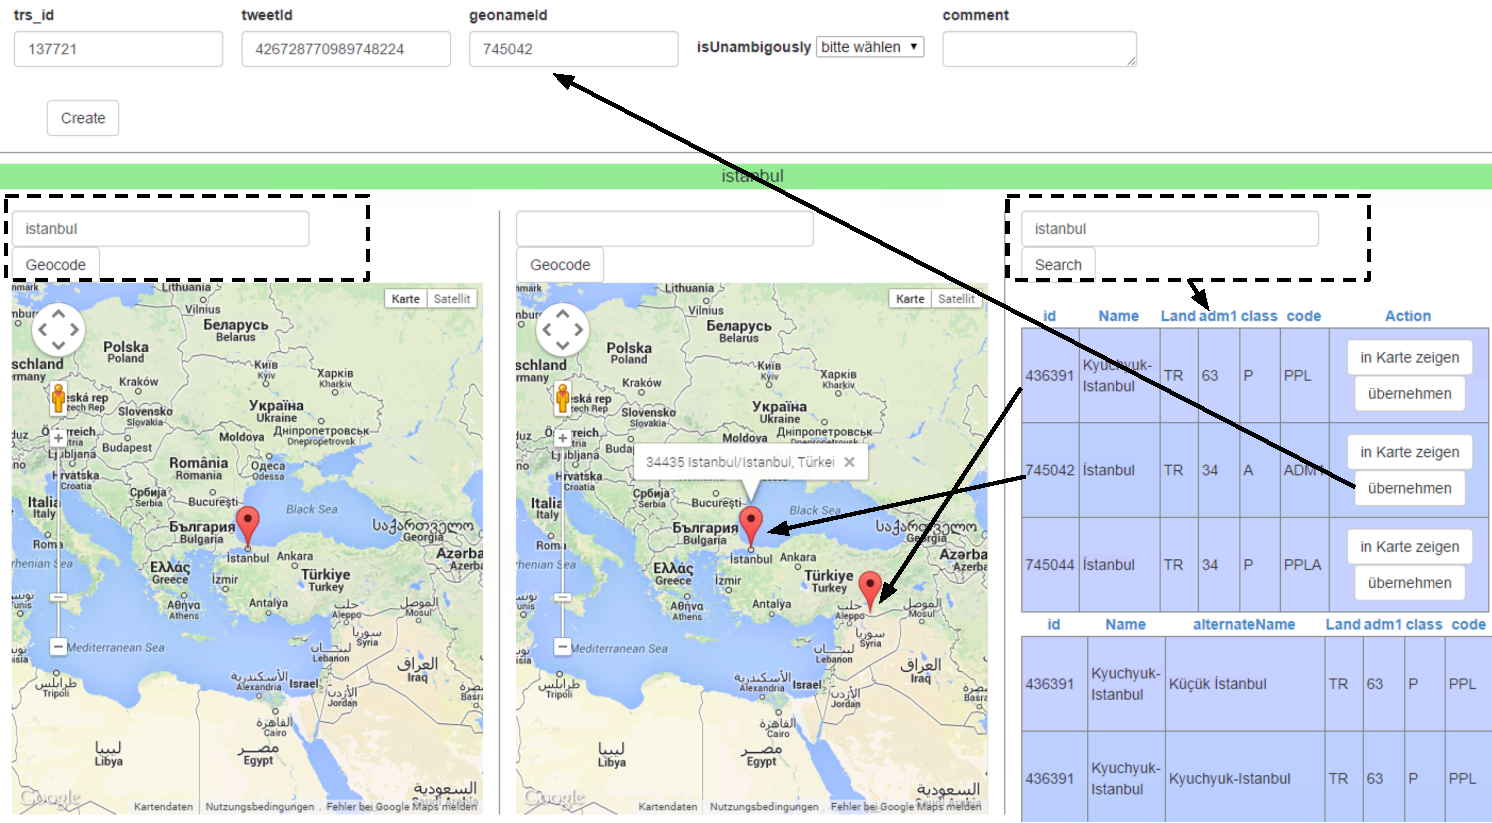
\includegraphics[scale=0.5]{_oberflaecheQuantitative.pdf}
						\caption{Oberfläche zur Untersuchung des Nutzer-Standortes}
						\label{img:oberflaecheQuantitative}
					\end{center}  
			\end{figure}	

			Die mit dieser Oberfläche erhobenen Daten wurden untersucht. 
			Die Ergebnisse werden in den folgenden Abschnitten vorgestellt.
			Es wurde über Google-Maos und geonames.org versucht, den Nutzer-Standort zuzuordnen. 
			Auch wenn die Sprache oder das verwendete Alphabet nicht bekannt, waren wurde eine Georeferenz zugeordnet, sofern die Suche auf den Ortsverzeichnissen einen Treffer ergab. 

		\subsection{Geografischer Bezug des Nutzer-Standortes} 
			
			In den eigenen Untersuchungen konnten 76\% der Nutzer-Standorte ein geografischer Bezug nachgewiesen werden. 
			Wurde geografischer Bezug nachgewiesen, so musste der Wert des Nutzer-Standortes im Ortsverzeichnis von geonames.org vorkommen. 
			Daraus kann gefolgert werden, dass in 76\% der Fälle ein Toponym im Nutzer-Standort vorhanden ist.
			
			In den restlichen 24\% der Fälle konnte kein geografischer Bezug mit Hilfe der Ortsverzeichnisse nachgewiesen werden. 
			Dies bedeutet nicht, dass grundsätzlich kein geografischer Bezug vorhanden ist. 
			Es konnte lediglich anhand der genutzten Quellen kein geografischer Bezug hergeleitet werden.
			Beispielsweise wurde "'Swag City"', ein Beiname für die Stadt "'Ann Arbor"', denn der Spitzname für die Stadt war in den Datenbanken nicht hinterlegt. 
			Dies zeigt, dass diesen Werten über ein Ortsverzeichnis keine Georeferenz zugewiesen werden konnte, durchaus aber geografischen Bezug haben können.
			Das Verwerfen solcher Werte durch unzureichendes Wissen über Toponyme kann zum Verlust wertvoller Informationen über den tatsächlichen Standort führen.

			Hecht et al. konnten in \cite{Hecht2011} den Datenwerten in den Nutzer-Standorten in 80\% der Fälle einen geografischen Bezug feststellen.
			In den restlichen 20\% der Fälle konnte im Nutzer-Standort kein geografischer Bezug festgestellt werden. 
			Diese Ergebnisse decken sich mit den eigenen Untersuchungen. 
			Es ist allerdings zu beachten, dass Hecht et al. ausschließlich Tweets aus den USA verwendet haben und die Nutzer-Standorte nur in englischer Sprache verfasst waren. 
					
	\section{Herausforderungen bei der Verwendung des Nutzer-Standortes als geografischen Indikator} \label{sec:HerausforderungenBeiDerVerwendungDesNutzerStadortes}  

		Neben den in Kapitel \ref{sec:zuordnungToponymeGeogObj} erwähnten Problemen bei der Zuordnung von Toponymen zu geografischen Objekten sind noch weitere Probleme zu erwarten.
		Diese sind hauptsächlich bedingt durch die freie Eingabe des Nutzer-Standortes.
		Es wurden dabei folgende Klassen identifiziert, in die die Werte eingeteilt werden können:

		\begin{enumerate}	
		 	\item Partieller geografischer Bezug des Wertes
		 	\item Widersprüchliche Werte 
		 	\item Geografische Hierarchien
		 	\item Domänenspezifische Toponyme (Neologismen)
		 	\item Toponyme unterschiedlicher Hierarchieebenen
		 	\item Keiner oder mittelbarer geografischer Bezug
		\end{enumerate}	 

		\subsection{Partieller geografischer Bezug des Datenwertes im Nutzer-Standort} \label{sub:partiellerGeografischerBezug} 

			Hierbei haben nur Teile des Wertes im Nutzer-Standort geografischen Bezug. 
			Im Nutzer-Standort werden oft weitere Informationen angegeben, die keinen geografischen Bezug haben. 
			Im Folgenden einige Beispiele.

			\begin{table}[h]
				\centering
				\caption{Beipiele für Nutzer-Standorte mit partiellem geografischen Bezug}
				\label{tab:partiellerGeogrBezug}
				\begin{tabular}{|l|l|l|}
				\hline
				\multicolumn{1}{|c|}{Wert} & \multicolumn{1}{c|}{geografischer Bezug} & \multicolumn{1}{c|}{kein geografischer Bezug} \\ \hline
				East side of that London & East side London & of that \\ \hline
				11th Dimension California & California & 11th Dimension \\ \hline
				New Orleans Home of the goons & New Orleans & Home of the goons \\ \hline
				Between here and there Miami & Miami & Between here and there \\ \hline
				\end{tabular}
			\end{table}
			
			Es können also auch nur Teile des Nutzer-Standorts für eine Geolokalisierung von Nutzen sein.
			Diese Informationen müssen extrahiert werden, um einen Nutzen aus ihnen ziehen zu können. 

		\subsection{Widersprüchliche Toponyme im Nutzer-Standort} \label{sub:wiederspruechlicheBezuege} 

			Es existieren auch Datenwerte, in denen mehrere widersprüchliche Angaben gemacht werden.
			Dies bedeutet, es werden zwei oder mehr Datenwerte mit geografischem Bezug angegeben, die auf unterschiedliche geografische Objekte verweisen.
			Auch hier sollen einige Beispiele genannt werden:

			\begin{table}[h]
			\centering
			\caption{Beispiele für widersprüchliche Toponyme}
			\label{tab:wiederspruechlicheBezuege}
			\begin{tabular}{|l|l|l|l|}
			\hline
			\multicolumn{1}{|c|}{Wert}      & \multicolumn{1}{c|}{Toponym 1} & \multicolumn{1}{c|}{Toponym 2} & \multicolumn{1}{c|}{Entfernung in km} \\ \hline
			Bolton\textbackslash/Leigh      & Bolton                         & Leigh                          & 14 									\\ \hline
			Liverpool\textbackslash/London  & Liverpool                      & London                         & 350 								\\ \hline
			Balikesir \textbackslash/ Izmir & Balikesir                      & Izmir                          & 180 								\\ \hline
			\end{tabular}
			\end{table}					
				
			In diesen Beispielen sind jeweils zwei Städte angegeben.

			Es kann nun spekuliert werden, wieso der Nutzer zwei Städte angibt.
			Ist er in einer der Städte aufgewachsen und lebt momentan in der anderen?
			Pendelt er zwischen den Städten um zu arbeiten?

			Es kann hier nicht eindeutig entschieden werden, in welcher Stadt sich der Nutzer aufhält.

		\subsection{Geografische Hierarchien im Nutzer-Standort} \label{sub:geografischeHierarchienImNutzerStandort} 

			Es ist auch möglich, dass im Nutzer-Standort Teile einer geografischen Hierarchie angegeben sind.
			Beispielsweise die Angabe einer Stadt in Kombination mit einem Land.
			
			In den USA wird beispielsweise oft die Stadt und der zugehörige Bundesstaat angegeben.
			In Brasilien hingegen wird oft ein Bundesstaat und das Land angegeben.
			Hier einige Beispiele:

			\begin{table}[h]
			\centering
			\caption{Beispiele für Nutzer-Standorte mit geografischen Hierarchieebenen}
			\label{tab:geografischeHierarchie}
			\begin{tabular}{|l|c|c|c|c|}
			\hline
			\multicolumn{1}{|c|}{Wert} & Stadt       & \multicolumn{1}{l|}{Adm2} & Adm1 & \multicolumn{1}{l|}{Land} \\ \hline
			Orange County, USA 		   & - 			 & Orange County										 & - 							   & USA    					\\ \hline
			Las Vegas, USA 		       & Las Vegas   & - 												     &								   & USA 					    \\ \hline
			Mato Grosso, Brazil        & -           & -                                                     & Mato Rrosso                     & Brazil                    \\ \hline
			West Sussex, England       & -           & -                                                     & West Sussex                     & England                   \\ \hline
			\end{tabular}
			\end{table}
 
			Durch die Kombination mehrerer Toponyme unterschiedlicher geografischer Hierarchieebenen wird die geografische Position näher beschrieben.
			Umso genauer eine geografische Position mit Toponymen beschrieben wird, umso geringer ist die Gefahr von Doppel- und Mehrdeutigkeiten.  
			Diese Information sollte bei einer Untersuchung erhalten bleiben.
			
		\subsection{Domänenspezifische Toponyme im Nutzer-Standort (Neologismen)} \label{sub:domaenenspezBezug} 

			In sozialen Netzwerken können sich eigene Begriffe und Formulierungen etablieren. 
			Diese sind im allgemeinen nicht bekannt.


			Im Twitter-Umfeld haben sich in den letzten Jahren einige spezielle Begriffe und Formulierungen zur Verwendung in Tweet-Texten etabliert. 
			Das im Twitter-Umfeld auch spezielle Toponyme im Nutzer-Standort verwendet werden, kann nicht gänzlich ausgeschlossen werden. 

			Ein Beispiel hierfür ist "'Bieberville"', welches in den untersuchten Daten von Hecht et al. öfter vorkommt \cite{Hecht2011}.
			"'Bieberville"' wird abgeleitet von dem Pop-Star Justin Bieber.	
			Da der Pop-Star in Twitter sehr aktiv ist und deshalb viele seiner Fans auch in Twitter aktiv sind hat sich dieser Name etabliert.
			Unter diesem Gesichtspunkt hätte "'Bieberville"' keinen geografischen Bezug.
			Sucht man im Internet nach "'Bieberville"' stößt man auf einen Imbiss in Groß-Bieberau.
			"'Bieberville"' kann also durchaus einen geografischen Bezug haben, wenngleich es im Twitter-Umfeld nicht als solcher benutzt wird. 
			Ist in einem Ortsverzeichnis beispielsweise "'Bierberville"' als Bezeichnung für den Imbiss in Groß-Bieberau hinterlegt, würde dieser als Georeferenz zugeordnet werden, was im Umfeld von Twitter in einem Großteil der Fälle falsch wäre.

			Das Wissen über die Verwendung domänenspezifischer Toponyme kann nur aus der Domäne selbst generiert.
		
		\subsection{Kein geografischer oder mittelbar geografischer Bezug} \label{sub:keinGeogOdMittelBarereBezug}

			Im Nutzer-Standortfeld können auch Werte auftauchen, die keinen geografischen Bezug aufweisen.
			Beispiele hierfür sind:

			\begin{table}[h]
			\centering
			\caption{Werte ohne oder mit mittelbarem geografischen Bezug}
			\label{tab:keinOderMittelbarBezug}
			\begin{tabular}{|l|}
			\hline
			Werte                      	\\ \hline
			In the middle of nowhere   	\\ \hline
			95                         	\\ \hline
			Highsociety                	\\ \hline
			cold	                 	\\ \hline
			rabbit     					\\ \hline
			\end{tabular}
			\end{table}

			Diese Werte haben auf den ersten Blick keinen geografischen Bezug.
			Es ist jedoch nicht auszuschließen, dass einige dieser Begriffe in bestimmten Regionen gehäuft auftreten.
			Damit hätten diese Begriffe geografischen Bezug.
			Dies kann bedingt durch die Landessprache oder Dialekte der Fall sein.

	\section{Verfahren zum Einlernen der Georeferenz-Basis} \label{sec:VefrahrenZumEinlernen} 	

			
			In Abbildung \ref{img:einlernenAblauf} ist der Gesamtablauf des Einlernens dargestellt. 
			Die Werte im Nutzer-Standortfeld werden zuerst einer Vorverarbeitung unterzogen. 
			Durch die Vorverarbeitung werden die Datenwerte im Nutzer-Standort vorbereitet, um weitere Informationen zu extrahieren.
			Es wird danach eine Zerlegung der Werte im Nutzer-Standortfeld vorgenommen.
			Die Zerlegung extrahiert dabei zusätzliche Informationen aus dem Nutzer-Standort.
			Die Nutzer-Zeitzone wird hinzugezogen, um bei der Geolokalisierung etwaige Doppel- und Mehrdeutigkeiten von Toponymen erkennen zu können.
			Das Ergebnis dieser Schritte ist eine Menge an Referenzwerten.

			\begin{figure}[!htb]
				\begin{center}
					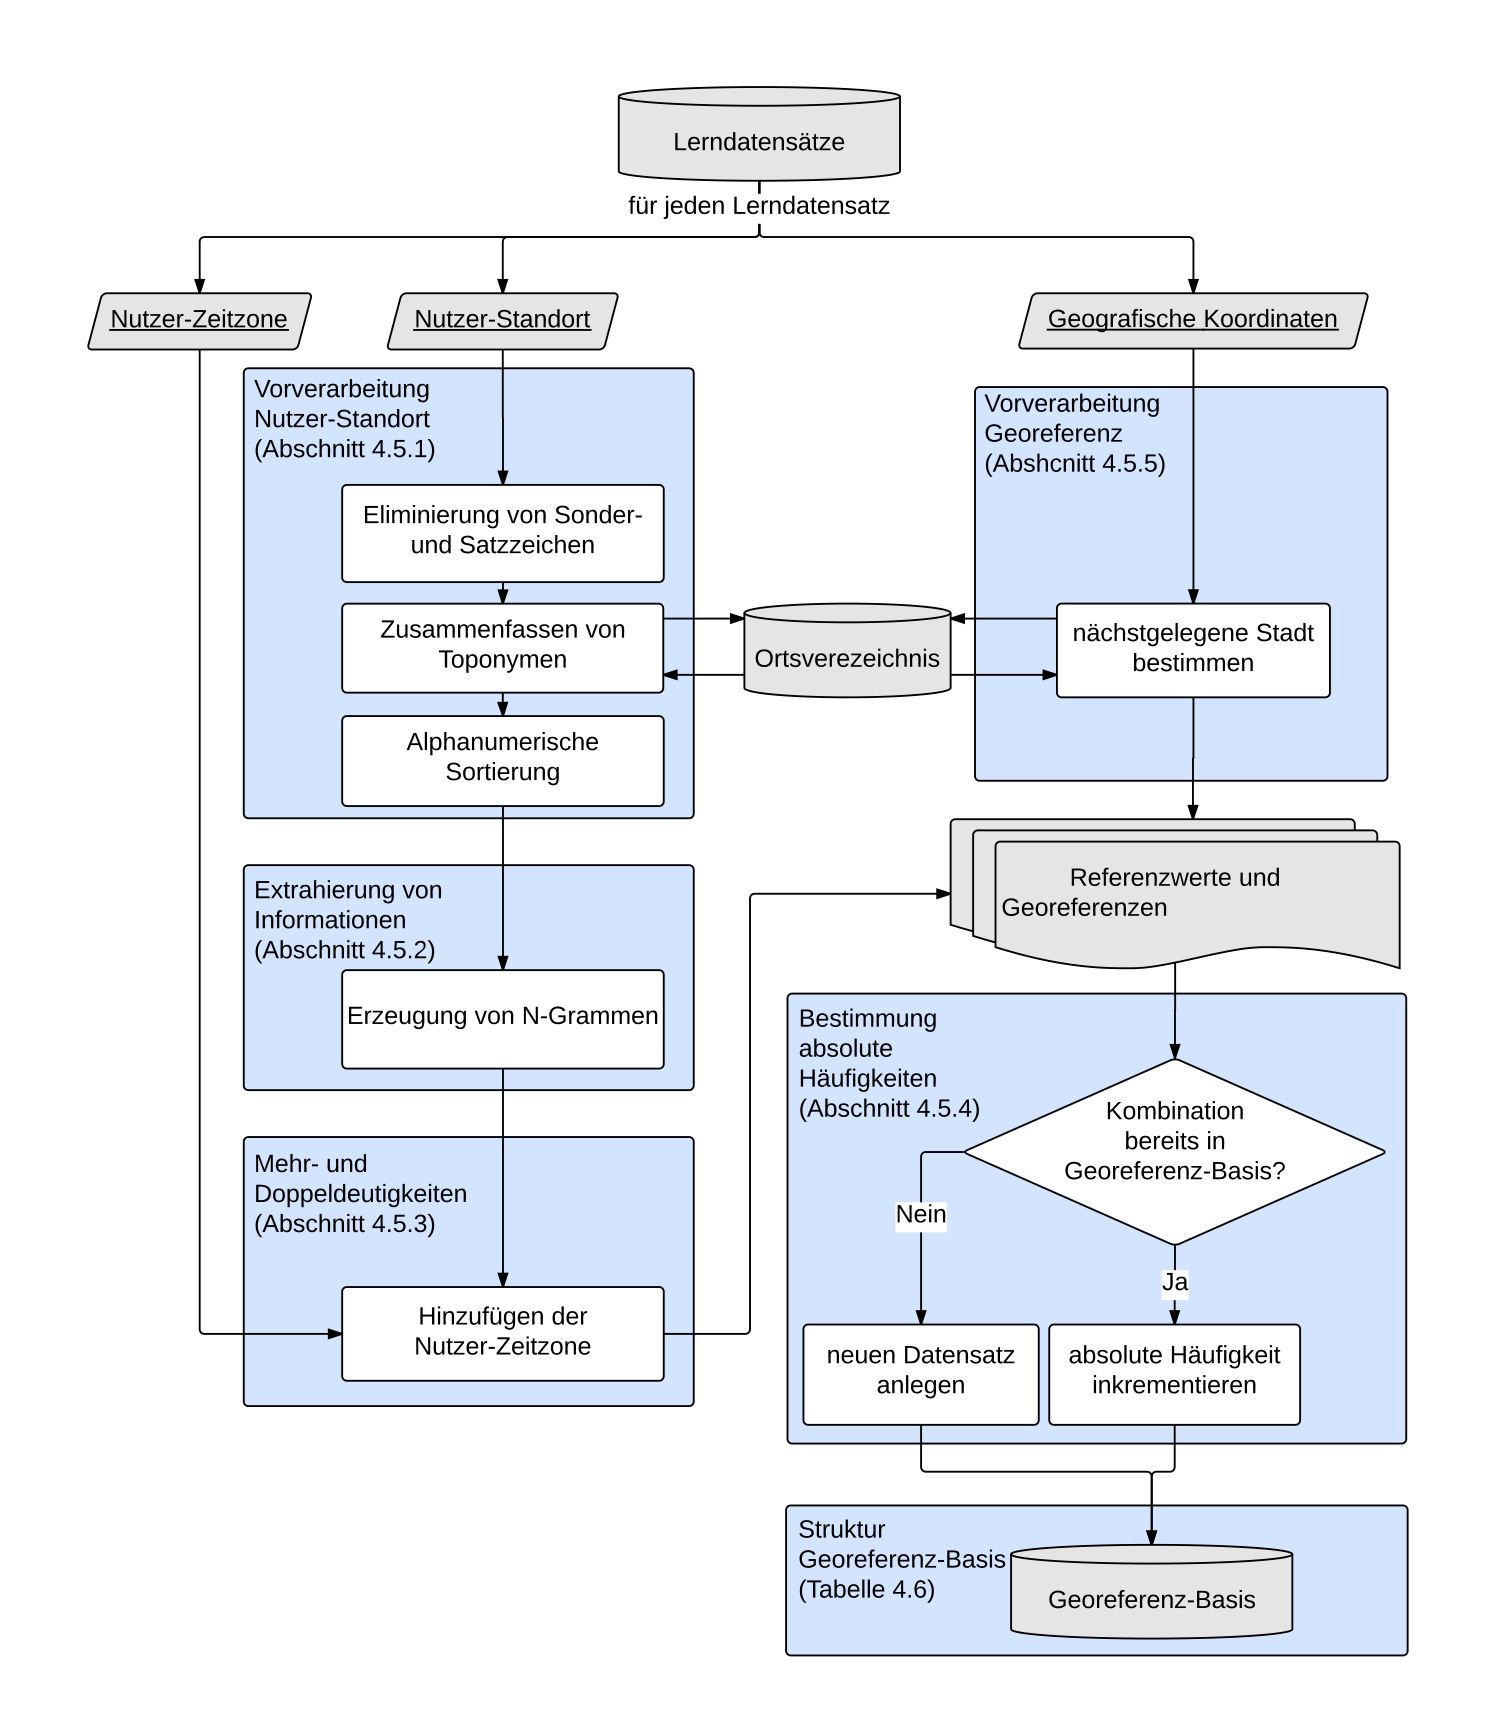
\includegraphics[scale=0.5]{einlernenAblauf.png}
					\caption{Ablaufplan einlernen}
					\label{img:einlernenAblauf}
				\end{center}
			\end{figure}
			\clearpage

			Parallel dazu werden die geografischen Koordinaten des Tweets auf eine diskrete geografische Position aufgelöst.
			Dies erfolgt durch die Zuordnung der geografischen Koordinaten zu der nächstgelegenen Stadt.

			Die Kombinationen aus Referenzwerten und diskreten geografischen Positionen werden in der Georeferenz-Basis gespeichert.
			Es wird dabei die quantitative Verteilung der Referenzwerte über den Globus erfasst.
			
			Die Datenstruktur der Georeferenz-Basis beinhaltet die Referenzwerte, die zugeordnete Stadt, und die übergeordneten Hierarchieebenen. 
			Zusätzlich wird das Vorkommen eines Referenzwertes in einer Stadt als absolute Häufigkeit gespeichert. 

			Durch dieses Verfahren lässt sich eine Datenbasis erzeugen, die auch domänenspezifische Eigenheiten berücksichtigt.
			Auch geografische Indikatoren mit mittelbarem geografischen Bezug, zum Beispiel die Verwendung spezieller Begriffe in einer geografischen Region, können einbezogen werden.

			In Tabelle \ref{tab:strukturMitHierarchie1} ist die Struktur der Georeferenz-Basis dargestellt.

			\begin{table}[htb]
				\caption{Struktur der Georeferenz-Basis mit geografischer Hierarchie} 
				\centering
				\tiny
				\begin{tabular}{|c|c|c|c|c|c|}
					\hline
					Referenzwert & Stadt & Adm2 & Adm1 & Land & abs. Häufigkeit \\
					\hline\hline
					 "'LA"' & Los Angeles & LA County & CA & USA & 30 \\
					\hline
					 "'San Francisco"'   & San Francisco & SF County & CA & USA & 3 \\
					\hline
					 "'Los Angeles"'   & Los Angeles & LA County & CA & USA & 70 \\
					\hline
					 "'Stuttgart"'   & Stuttgart & Regierungsbezirk Stuttgart & BaWü & BRD & 80 \\
					\hline
					 "'London City"'   & London & City London & Greater London & GB & 90\\
					\hline
				\end{tabular}
				\label{tab:strukturMitHierarchie1} 
			\end{table}  

			

		\subsection{Schritte zur Vorverarbeitung der Werte des Nutzer-Standortfeldes} \label{sub:Vorv}

			Die Werte des Nutzer-Standortfeldes werden einer Vorverarbeitung unterzogen.
			In Abbildung \ref{img:vorverarbeitung} sind die einzelnen Schritte dargestellt.
			Die Vorverarbeitung ist notwendig um die Werte auf die Extrahierung weiterer Daten vorzubereiten.
			Die einzelnen Worte im Nutzer-Standort werden als Token bezeichnet. 
			
			Es sollen zunächst Sonder- und Satzzeichen entfernt werden.
			Diesen kann in der Regel kein geografischer Bezug nachgewiesen werden.
			In einem weiteren Schritt werden mit Hilfe eines Ortsverzeichnisses zwei oder mehr Token, die gemeinsam ein Toponym darstellen, zusammengefasst.
			Danach wird eine alphanumerische Sortierung der Token durchgeführt.

			In Tabelle \ref{tab:VorverarbeitungBsp1} sind einige Werte von Nutzer-Standortfeldern aufgeführt.
			Diese sollen in den folgenden Abschnitten als durchgängiges Beispiel verwendet werden.

				\begin{table}[h]
					\centering
					\caption{Beispielwerte}
					\label{tab:VorverarbeitungBsp1}
					\begin{tabular}{|l|l|}
					\hline 
					\multicolumn{2}{|c|}{\textbf{Werte Nutzer-Standortfeld}} \\ \hline \hline
					1&Mato Grosso \& Rio de Janeiro                      			\\ \hline
					2&\_***\_                                         			\\ \hline
					3&USA\textbackslash /Los Angeles                  			\\ \hline
					4&Los Angeles, USA                                			\\ \hline
					5&$\dagger$\textasciitilde York \textasciitilde$\dagger$      \\ \hline
					6&Nottingham\textbackslash /London                			\\ \hline
					7&York                                            			\\ \hline
					8&11th Dimension | California 					\\ \hline	
					\end{tabular}
				\end{table} 
			 
			\subsubsection{Eliminierung von Sonder- und Satzzeichen} 

				Es werden oft Sonder- und Satzzeichen im Nutzer-Standort verwendet. 
				Beispielsweise als Trenner zwischen Toponymen unterschiedlicher geografischer Hierarchieebenen.
				Beispiele hierfür sind die Zeilen 1,3 und 6 in Tabelle \ref{tab:VorverarbeitungSonder}. 
				Die Trennzeichen werden nicht einheitlich verwendet.
				Weder die Rangfolge der Hierarchieebene noch das verwendete Satzzeichen sind einheitlich.  
				Es ist also nicht klar welcher Zusammenhang zwischen den Datenwerten, die durch ein Sonder- oder Satzzeichen getrennt werden, besteht. 

				Auch werden Sonder- und Satzzeichen ausschließlich oder als Dekoration verwendet.
				Beispiele hierfür sind die Zeilen 2 und 5 in Tabelle \ref{tab:VorverarbeitungSonder}.
				In den oben genannten Fällen bringen Sonder- und Satzzeichen keine zusätzlichen Informationen.
				Es sollen deshalb in einem ersten Vorverarbeitungsschritt alle Sonder- und Satzzeichen entfernt werden. 

				Liste nach dem Entfernen von Sonder- und Satzzeichen:

				\begin{table}[h]
				\centering
				\caption{Eliminierung von Sonder- und Satzzeichen}
				\label{tab:VorverarbeitungSonder}
				\begin{tabular}{|l|l|l|}
				\hline 
				  & \multicolumn{1}{c|}{\textbf{Vorher}} & \multicolumn{1}{c|}{\textbf{Nachher}} \\ \hline \hline
				1 & Mato Grosso \& Rio de Janeiro        & Mato Grosso Rio de Janeiro            \\ \hline
				2 & \_***\_                              &                                       \\ \hline
				3 & USA\textbackslash /Los Angeles       & USA Los Angeles                       \\ \hline
				4 & Los Angeles, USA                     & Los Angeles USA                       \\ \hline
				5 & $\dagger$\textasciitilde York \textasciitilde$\dagger$                             & York                                  \\ \hline
				6 & Nottingham\textbackslash /London     & Nottingham London                     \\ \hline
				\end{tabular}
				\end{table}

				Der Wert in Zeile 6 existiert nun nicht mehr, der Wert ist leer und wird somit nicht weiter betrachtet.

			\subsubsection{Zusammenfassen von Toponymen mit Hilfe von a priori Wissen aus einem Ortsverzeichnis}

				Oft bestehen Toponyme aus zwei oder mehr Token.
				Diese sollen mit Hilfe eines Ortsverzeichnisses zusammengefasst werden. 
				Dies kann selbstverständlich nur für bekannte Toponyme durchgeführt werden.
				
				"'Los"' und "'Angeles"' bilden gemeinsam "'Los Angeles"' und sollen in der weiteren Verarbeitung gemeinsam betrachtet werden. 
				Dies soll zunächst mit einem + Zeichen gekennzeichnet werden.

				Daraus resultiert:

				\begin{table}[h]
				\centering
				\caption{Zusammenfassen von Toponymen}
				\label{tab:VorverarbeitungZusammen}
				\begin{tabular}{|l|l|l|}
				\hline
				  & \multicolumn{1}{c|}{\textbf{Vorher}} & \multicolumn{1}{c|}{\textbf{Nachher}} \\ \hline \hline
				1 & Mato Grosso Rio de Janeiro           & Mato+Grosso Rio+de+Janeiro            \\ \hline
				2 &                                      &                                       \\ \hline
				3 & USA Los Angeles                      & USA Los+Angeles                       \\ \hline
				4 & Nottingham London                    & Nottingham London                     \\ \hline
				5 & Los Angeles USA                      & Los+Angeles USA                       \\ \hline
				6 & York                                 & York                                  \\ \hline
				7 & 11th Dimension California            & 11th Dimension California             \\ \hline
				\end{tabular}
				\end{table}

				In diesem Schritt wird keine Geolokalisierung vorgenommen.
				Es werden lediglich Toponyme die aus zwei oder mehr Token bestehen identifiziert.
				Er dient dazu, möglichst früh vorhandenes Wissen über Toponyme einzubeziehen und zusammengehörige Toponyme in den nächsten Schritten als ein Token zu behandeln.

			\subsubsection{Angleichung durch alphanumerische Sortierung}

				In diesem Schritt sollen die Token alphanumerisch sortiert werden. 
				Wenn Toponyme unterschiedlicher geografischer Hierarchieebenen angegeben sind, spielt es keine Rolle mehr, in welcher Reihenfolge diese angegeben werden.

				\begin{table}[h]
				\centering
				\caption{Alphanumerische Sortierung}
				\label{tab:VorverarbeitungAlpha}
				\begin{tabular}{|l|l|l|}
				\hline
				  & \multicolumn{1}{c|}{\textbf{Vorher}} & \multicolumn{1}{c|}{\textbf{Nachher}} \\ \hline
				1 & Mato+Grosso Rio+de+Janeiro           & Mato+Grosso Rio+de+Janeiro            \\ \hline
				2 &                                      &                                       \\ \hline
				3 & USA Los+Angeles                      & Los+Angeles USA                       \\ \hline
				4 & Nottingham London                    & London Nottingham                     \\ \hline
				5 & Los+Angeles USA                      & Los+Angeles USA                       \\ \hline
				6 & York                                 & York                                  \\ \hline
				7 & 11th Dimension California            & 11th California Dimension             \\ \hline
				\end{tabular}
				\end{table}

				In den Zeilen 3 und 5 in Tabelle \ref{tab:VorverarbeitungAlpha} ist nun die Reihenfolge der Toponyme angeglichen. 
				
				Dieser Schritt stellt einen Kompromiss dar.
				Es werden zwar Werte mit gleichem Inhalt und unterschiedlicher Reihenfolge angeglichen.
				Aber es werden auch potenzielle Toponyme, die aus mehreren Token bestehen, auseinandergezogen.
				Als Beispiel soll hier "'Motor City Michigan USA"' betrachtet werden.
				Wenn "'Motor City"' nicht im Ortsverzeichnis hinterlegt ist, entsteht durch die alphanumerische Sortierung "'City Michigan Motor USA"'.
				Der Zusammenhang zwischen Motor und City wäre nicht mehr vorhanden und kann nicht wiedergewonnen werden.

		\subsection{Zerlegung der Werte im Nutzer-Standortfeld} \label{sub:VorvNGramme}

			Als Eingabe wird in diesem Schritt das Ergebnis der Vorverarbeitung genutzt. 
			Pro Nutzer-Standortfeld existieren ein oder mehrere Token. 
			Ist nur ein Token vorhanden, so wird dieser direkt weiter verarbeitet.
			Sind mehrere Token vorhanden, so können diese partiellen geografischen Bezug aufweisen (siehe Abschnitt \ref{sub:partiellerGeografischerBezug}) oder eine Hierarchie darstellen (siehe Abschnitt \ref{sub:geografischeHierarchienImNutzerStandort}).
			Durch die Zerlegung sollen einzelne Token für die Weiterverarbeitung extrahiert werden.
			In diesem Fall soll es ermöglicht werden, Token mit geografischem Bezug von solchen ohne geografischen Bezug zu trennen, um diese separat weiterverarbeiten zu können.
			Um allerdings die zusätzlichen Informationen, die durch die Angabe einer geografischen Hierarchie entstehen zu erhalten, sollen auch mehrere Token gemeinsam weiterverarbeitet werden können.
			Das bedeutet, der Zusammenhang mehrere Token, die in einer gewissen Reihenfolge auftreten, soll erhalten bleiben. 
			Um dies zu erzielen, werden die Token in sogenannte N-Gramme zerlegt. 

			\subsubsection{N-Gramme} 

				Eine Gruppe von Token soll derart zerlegt werden, dass sowohl einzelne Token betrachtet werden können, als auch der Zusammenhang zwischen den Token, der durch ihre Reihenfolge  besteht, erhalten bleibt.
				Um dies umzusetzen, wird eine Menge von Token in N-Gramme zerlegt werden.

				Die Zerlegung in N-Gramme findet unter anderem Anwendung in der Computerlinguistik und quantitativen Linguistik.
				N-Gramme bestehen aus ein oder mehreren Wörtern, die aus einem Text extrahiert werden. 
				Im vorliegenden Fall sollen die Token aus dem Nutzer-Standortfeld betrachtet werden.
				Die Extrahierung erfolgt dabei derart, dass immer zwei oder mehr aufeinanderfolgende Token zusammengefasst werden.    
				Ein Spezialfall sind Uni-Gramme, hierbei wird die Menge an Token in die einzelnen Token zerlegt.
				Bi-Gramme bestehen aus jeweils zwei aufeinanderfolgenden Token.
				Tri-Gramme bestehen aus drei aufeinanderfolgenden Token. 
				Die Anzahl der Token aus der ein N-Gramm besteht, wird auch Grad des N-Grammes genannt.

				In Tabelle \ref{tab:ngramize} wird der Ablauf zur Erzeugung von N-Grammen bis zum Grad 3 Schrittweise dargestellt.
				In Schritt 1,2 und 3 werden Uni-Gramme erzeugt. 
				Diese bestehen jeweils aus einem Token.
				In den Zeilen 4 und 5 sind die beiden Bi-Gramme dargestellt.
				In Zeile 6 schließlich wird das Tri-Gramm dargestellt. 

				\begin{table}[h]
				\centering
				\caption{Beispiel zur Erzeugung von N-Grammen}
				\label{tab:ngramize}
				\begin{tabular}{|c||l|l|l||l|}
				\hline
				 & \multicolumn{1}{c|}{0}    & \multicolumn{1}{c|}{1}         & \multicolumn{1}{c|}{2}          & Ordnung \\ \hline \hline
				0       & 11th                      & Dimension                      & California                      & -       \\ \hline
				1       & \textless 11th \textgreater &                                &                                 & 1       \\ \hline
				2       &                           & \textless Dimension\textgreater &                                 & 1       \\ \hline
				3       &                           &                                & \textless California\textgreater & 1       \\ \hline
				4       & \textless 11th\textgreater & \textless Dimension\textgreater &                                 & 2       \\ \hline
				5       &                           & \textless Dimension\textgreater & \textless California\textgreater & 2       \\ \hline
				6       & \textless 11th\textgreater & \textless Dimension\textgreater & \textless Calforinia\textgreater & 3       \\ \hline
				\end{tabular}
				\end{table}

				 
				
				In Tabelle \ref{tab:NGramme} sind alle N-Gramme zu den Beispielen aus Tabelle \ref{tab:VorverarbeitungAlpha} dargestellt.

					\begin{table}[h]
					\centering
					\caption{Zerlegung in N-Gramme}
					\label{tab:NGramme}
					\begin{tabular}{|l|l|l|}
					\hline 
					\multicolumn{1}{|c|}{\textbf{}} & \multicolumn{1}{c|}{\textbf{Vorher}}        & \multicolumn{1}{c|}{\textbf{Nachher}}                                                    \\ \hline \hline
					\multirow{3}{*}{1}              & \multirow{3}{*}{Mato+Grosso Rio+de+Janeiro} & \textless Mato+Grosso\textgreater\textless Rio+de+Janeiro\textgreater                     \\ \cline{3-3} 
					                                &                                             & \textless Mato+Grosso\textgreater                                                         \\ \cline{3-3} 
					                                &                                             & \textless Rio+de+Janeiro\textgreater                                                     \\ \hline \hline
					2                               &                                             &                                                                                          \\ \hline \hline
					\multirow{3}{*}{3}              & \multirow{3}{*}{Los+Angeles USA}            & \textless Los+Angeles\textgreater\textless USA\textgreater                                 \\ \cline{3-3} 
					                                &                                             & \textless Los+Angeles\textgreater                                                         \\ \cline{3-3} 
					                                &                                             & \textless USA\textgreater                                                                 \\ \hline \hline
					\multirow{3}{*}{4}              & \multirow{3}{*}{London Nottingham}          & \textless London\textgreater\textless Nottingham\textgreater                               \\ \cline{3-3} 
					                                &                                             & \textless London\textgreater                                                              \\ \cline{3-3} 
					                                &                                             & \textless Nottingham\textgreater                                                          \\ \hline \hline
					5                               & Los+Angeles USA                             &                                                                                          \\ \hline \hline
					6                               & York                                        & \textless York\textgreater                                                                \\ \hline \hline
					\multirow{6}{*}{7}              & \multirow{6}{*}{11th Dimension California}  & \textless 11th\textgreater\textless California\textgreater\textless Dimension\textgreater \\ \cline{3-3} 
					                                &                                             & \textless 11th\textgreater                                                                \\ \cline{3-3} 
					                                &                                             & \textless California\textgreater                                                         \\ \cline{3-3} 
					                                &                                             & \textless Dimension\textgreater                                                          \\ \cline{3-3} 
					                                &                                             & \textless 11th\textgreater\textless California\textgreater                                 \\ \cline{3-3} 
					                                &                                             & \textless California\textgreater\textless Dimension\textgreater                           \\ \hline
					\end{tabular}
					\end{table}

				Durch die Erzeugung von N-Grammen wird es ermöglicht, einzelne Token zu betrachten.
				Haben die Werte im Nutzer-Standortfeld nur partiellen geografischen Bezug, können diese getrennt voneinander weiterverarbeitet werden.
				In Tabelle \ref{tab:NGramme} in Zeile 7 ist dies beispielsweise der Wert "'California"', de getrennt von "'11th"' und "'Dimension"' betrachtet werden kann. 
				
				Tauchen widersprüchliche Toponyme in einem Nutzer-Standortfeld auf, so können auch diese getrennt voneinander weiterverarbeitet werden.

				In Zeile 3 und 5 bleibt die Hierarchiebeziehung der Token im Bi-Gramm erhalten.
				Aber es können auch die einzelnen Werte mit geografischem Bezug weiter verarbeitet werden, da aus den Toponymen "'Los+Angeles"' und "'USA"' auch Uni-Gramme erzeugt werden.
				Der Vorteil der Zerlegung durch N-Gramme besteht darin, dass Token einzeln oder im Zusammenhang betrachtet werden können. 
				Somit kann aus einer Menge Token mehr Information extrahiert werden.

			\subsubsection{Weitere Verwendung der entstandenen N-Gramme} 

				Es kann zu diesem Zeitpunkt maschinell keine Entscheidung getroffen werden, ob eines der N-Gramme einen geografischen Bezug aufweist oder nicht.
				Eine Entscheidung darüber würde erfordern, a priori Wissen über den geografischen Bezug der N-Gramme einzubeziehen. 
				Dies ist allerdings aufgrund der Vielfalt und der möglicherweise auftauchenden Werte mit mittelbarem geografischen Bezug kaum möglich. 
				Da hier maschinell keine Entscheidung getroffen werden kann, welche Uni-, Bi- oder Tri-Gramme einen geografischen Bezug aufweisen, werden alle N-Gramme in die weitere Verarbeitung einbezogen. 			
				Es werden somit keine Token verworfen, denen aufgrund von unzureichenden Informationen, beispielsweise durch ein unvollständiges Ortsverzeichnis, keine Georeferenz zugeordnet werden kann.
				Auch werden Werte mit mittelbarem geografischen Bezug in die weitere Verarbeitung einbezogen.
				Token mit und ohne geografischen Bezug werden weiter verarbeitet.
				Eine Entscheidung über den geografischen Bezug wird erst während der Geolokalisierung getroffen.

		\subsection{Mehr- und Doppeldeutigkeiten} \label{sub:VorvNutzerZeitzone} 

				In Kapitel \ref{sec:zuordnungToponymeGeogObj} wurde auf die Probleme bei der Zuordnung von Toponymen zu geografischen Objekten eingegangen.
				Dabei wurde die Mehr- und Doppeldeutigkeit von Toponymen betrachtet.
				In den N-Grammen kann dieses Problem nach wie vor auftauchen.
				Dies ist genau dann der Fall, wenn ein N-Gramm ein Toponym darstellt.

				Um diesem Problem zu begegnen, wird die Nutzer-Zeitzone als weiterer geografischer Indikator hinzugezogen.

				Zunächst sollen die generellen Eigenschaften der Nutzer-Zeitzone erläutert werden bevor erklärt wird wie die Nutzer-Zeitzone das Problem der Mehr- und Doppeldeutigkeit von Toponymen beheben kann.

				\subsubsection{Eigenschaften der Nutzer-Zeitzone}

					Eine Zeitzone beschreibt eine eindeutige geografische Region auf dem Globus und hat somit unmittelbaren geografischen Bezug.
					Dabei entsprechen die Grenzen der Zeitzonen-Regionen nicht unbedingt den Landesgrenzen oder den Grenzen sonstiger Verwaltungseinheiten. 
					In Abbildung \ref{img:timezones} sind die Zeitzonen der Erde dargestellt.

					\begin{figure}[!ht]
						\begin{center}
							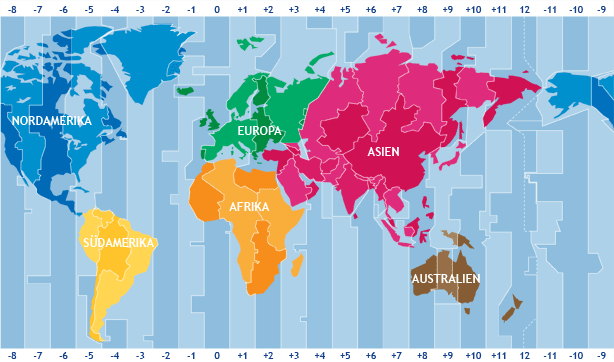
\includegraphics[scale=0.5]{zeitzonen_weltkarte.jpg}
							\caption{Zeitzonen der Erde.}
							\label{img:timezones}
						\end{center}
					\end{figure}	
					%Quelle: http://www.zeitzonen.de/images/frontend/mod\_tz\_map/zeitzonen\_weltkarte.gif

				\subsubsection{Eignung der Nutzer-Zeitzone zur Eliminierung von Mehr- und Doppeldeutigkeiten}

					In Abbildung \ref{img:usTimezones} wurden Tweets anhand ihres Längen- und Breitengrades platziert.
					Jeder Punkt in der Abbildung entspricht einem Tweet.
					Es wurden nur Tweets aus den USA ausgewählt.
					Anhand der Nutzer-Zeitzone wurde jedem Tweet eine Farbe zugeordnet.
					In Tabelle \ref{tab:timezoneColors} sind die Farbzuordnungen aufgelistet. 

					\begin{table}[h]
					\centering
					\caption{In Abbildung \ref{img:usTimezones} werden folgende Farben verwendet}
					\label{tab:timezoneColors}
						\begin{tabular}{|l|l|}
							\hline
							Zeitzone      & Farbe     \\ \hline \hline
							Pacific Time  & Rot       \\ \hline
							Eastern Time  & Grün/Gelb \\ \hline
							Central Time  & Blau      \\ \hline
							Mountain Time & Pink      \\ \hline
						\end{tabular}
					\end{table}

					 \begin{figure}[!ht]
						\begin{center}
							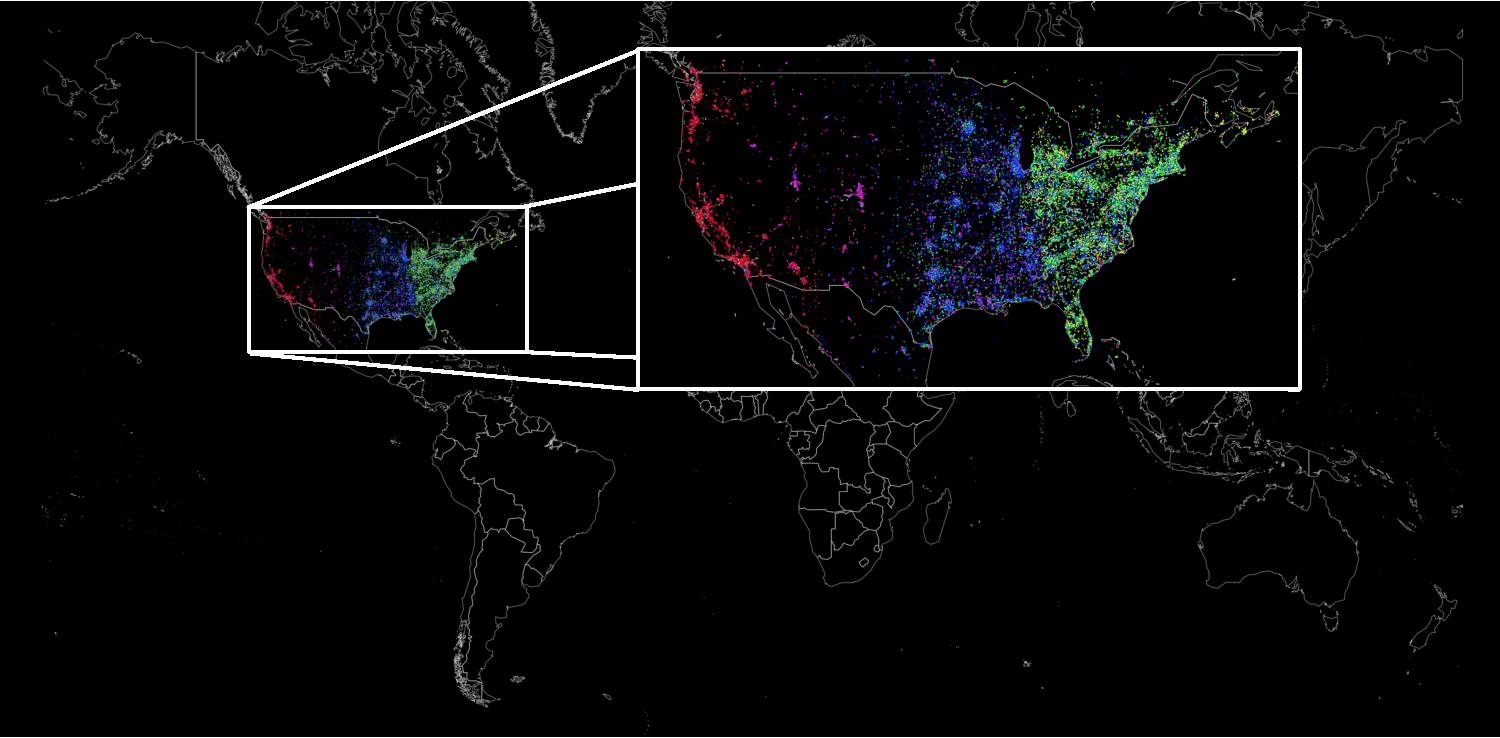
\includegraphics[scale=0.5]{usTimezones.pdf}
							\caption{Tweets, abhängig der Zeitzone eingefärbt}
							\label{img:usTimezones}
						\end{center}
					\end{figure}	

					Lediglich die dünn besiedelte Region der Mountain Time kann nur an einigen Ballungszentren erkannt werden. 
					Grundsätzlich scheint der Großteil der Angaben aber korrekt zu sein.

					Ist ein Toponym doppel- oder mehrdeutig kann nicht entschieden werden, welches geografische Objekt zugeordnet werden soll.
					Liegen die beiden geografischen Objekte allerdings in zwei unterschiedlichen Zeitzonen und der Nutzer hat die Nutzer-Zeitzone korrekt angegeben, kann die Doppeldeutigkeit aufgelöst werden.
					Voraussetzung hierfür ist natürlich, dass die geografischen Objekte in zwei unterschiedlichen Zeitzonen liegen und die Nutzer-Zeitzone angegeben ist.

				\textit{Hinzufügen der Nutzer-Zeitzone} 

					An die Referenzwerte, die aus dem Nutzer-Standort erzeugt wurden, wird nun die Zeitzone angehängt werden.
					Jeder Referenzwert soll einmal mit und einmal ohne Zeitzone existieren. 
					Damit wird garantiert, dass eingelernte Referenzwerte, die eine falsche Zeitzone aufweisen, trotzdem berücksichtigt werden können. 

					Um die Nutzer-Zeitzone von den aus dem Nutzer-Standort generierten Elementen unterscheiden zu können, wird die Nutzer-Zeitzone kursiv geschrieben.
					Auch hier wird die Liste weiter eingeschränkt und es werden lediglich noch zwei Beispiele betrachtet.
					
					\begin{table}[h]
					\centering
					\caption{Hinzufügen der Zeitzone}
					\label{tab:ngramsWithTZ}
					\begin{tabular}{|l|l|}
					\hline
					  & \textbf{Referenzwerte}                                                                     \\ \hline
					1 & \textless Los+Angeles\textgreater\textless USA\textgreater                                   \\ \hline
					2 & \textless Los+Angeles\textgreater                                                           \\ \hline
					3 & \textless USA\textgreater                                                                   \\ \hline
					4 & \textless Los+Angeles\textgreater\textless USA\textgreater\textless \textit{Pacific+Times}\textgreater \\ \hline
					5 & \textless Los+Angeles\textgreater\textless \textit{Pacific+Times}\textgreater               \\ \hline
					6 & \textless USA\textgreater\textless \textit{Pacific+Times}\textgreater                       \\ \hline
					7 & \textless York\textgreater                                                                  \\ \hline
					8 & \textless York\textgreater\textless \textit{London+Time}\textgreater                        \\ \hline
					\end{tabular}
					\end{table}

					Ein Beispiel für eine Auflösung der Doppeldeutigkeit ist in Tabelle \ref{tab:ngramsWithTZ} für das Token \textless York\textgreater  angegeben.
					Zum einen existiert "'York"' in England zum anderen in den USA.  
					Mit Hilfe der zusätzlichen Zeitzone können geografische Objekte, wenn sie in verschiedenen Zeitzonen liegen, unterschieden werden.

		\subsection{Bestimmung der absoluten Häufigkeiten der Referenzwerte} \label{sub:absHaufBestimmen} 

			Es werden nun die absoluten Häufigkeiten der Referenzwerte bestimmt.
			Dabei werden die Vorkommen der Referenzwerte an einer geografischen Position gezählt.
			Auf Basis dieser Werte wird die spätere Geolokalisierung ermöglicht.

			Jedes oben ermittelte N-Gramm und die Kombination aus N-Gramm und Zeitzone werden als einzelne Referenzwerte betrachtet. 
			Jedem Referenzwert werden die geografischen Koordinaten des Tweets zugeordnet, aus dem der Referenzwert erzeugt wurde.
			Zur Verdeutlichung ist in Tabelle \ref{tab:bspWerteAusEinemTweet} das Ergebnis der oben genannten Schritte an einem Beispiel dargestellt. 

				\begin{table}[h]
				\begin{tabular}{|l|l|l|}
				\hline
				\textbf{}         & Nutzer-Standortfeld:                                                                       & love Los Angeles                                                \\ \cline{2-3} 
				\textbf{Ursprung} & Nutzer-Zeitzone                                                                            & Pacific Time                                                    \\ \cline{2-3} 
				\textbf{}         & Geografische Koordinaten                                                                   & (33.78,118.29)                                                  \\ \hline
				                  & \multicolumn{1}{c|}{\textit{\textbf{Referenzwert}}}                                        & \multicolumn{1}{c|}{\textit{\textbf{geografische Koordinaten}}} \\ \hline
				1                 & \textless Los+Angeles\textgreater\textless love\textgreater                                  & (33.78, 118.29)                                                 \\ \hline
				2                 & \textless Los+Angeles\textgreater                                                           & (33.78, 118.29)                                                 \\ \hline
				3                 & \textless love\textgreater                                                                  & (33.78, 118.29)                                                 \\ \hline
				5                 & \textless Los+Angeles\textgreater\textless love\textgreater\textless Pacific+Time\textgreater & (33.78, 118.29)                                                 \\ \hline
				\textit{6}        & \textless Los+Angeles\textgreater\textless Pacific+Time\textgreater                          & (33.78, 118.29)                                      \\ \hline
				7                 & \textless Los+Angeles\textgreater\textless love\textgreater\textless Pacific+Time\textgreater & (33.78, 118.29)                                                 \\ \hline
				\end{tabular}
				\caption{Ergebnis für Love Los Angeles, Pacific Time}
					\label{tab:bspWerteAusEinemTweet}
				\end{table}


			Jeder Tweet aus den Trainingsdatensätzen wird in dieser Weise verarbeitet. 
			Es liegt damit eine Menge an Referenzwerten mit zugehörigen geografischen Koordinaten vor.

			Mit Hilfe dieser Daten wird nun die Georeferenz-Basis aufgebaut. 
			Für jedes Tupel wird in der vorgestellten Struktur der Georeferenz-Basis (siehe Tabelle \ref{tab:strukturMitHierarchie1}) ein Datensatz angelegt und mit einem Wert von 1 für die absolute Häufigkeit initialisiert. 
			Stimmt sowohl der Referenzwert als auch die geografische Position mit einem vorhandenen Datensatz überein, wird die absolute Häufigkeit für dieses Tupel inkrementiert.
			In dieser Art werden alle erzeugten Referenzwerte und geografischen Postionen verglichen, und die Anzahl der Vorkommen an einer geografischen Position erfasst.

			Die geografischen Koordinaten eines Tweets sind für diese Art der quantitativen Erfassung allerdings zu genau. 
			Der Längen- und Breitengrad wird meistens mit Hilfe von GPS-Modulen mobiler Endgeräte, wie Smartphones, erfasst.
			Diese geben eine Position oft auf wenige Meter genau an.
			Das bedeutet, zwei Tweets die wenige Meter voneinander abgesetzt wurden, haben in der Regel unterschiedliche Werte für den Längen- und Breitengrad.
			Dies kann für die Bestimmung der Häufigkeiten problematisch sein, da die Werte des Längen- und Breitengrades in der Regel nicht exakt übereinstimmen.
			Deshalb soll mit Hilfe der geografischen Koordinaten jeder Referenzwert der nächstgelegenen Stadt zugeordnet werden (siehe Abschnitt \ref{sub:Stadtbestimmen}).

		\subsection{Zuordnung der nächstgelegenen Stadt mit Hilfe von Voronoi-Regionen} \label{sub:Stadtbestimmen} 

			Um die geografischen Positionen der Referenzwerte vergleichbar zu machen, wird jeder Referenzwert auf die geografischen Koordinaten der nächstgelegenen Stadt abgebildet.
			Dies wird mit Hilfe von Voronoi-Diagrammen umgesetzt.

			In einem Voronoi-Diagramm ist eine Ebene und eine Menge an Punkten derart zerlegt, dass jedem Punkt eine Region zugeordnet wird, die sogenannten Voronoi-Regionen.
			In jeder dieser Region liegt dabei exakt ein Punkt.  

			Sei eine Menge von Punkten $Z = {z_1,z_2,...,z_n}$ auf einer Ebene verteilt.
			Eine Voronoi-Region $V^i$ zu einem Punkt $z_i$ beinhaltet dann alle Punkte $P^i={p_1,p_2,...,p_n}$ die näher an $z_i$ liegen als an allen anderen Punkten $Z_j={z_j in Z|z_j!=z_i}$.
			Alle Voronoi-Regionen zu allen Punkten in Z bilden ein Voronoi-Diagramm.

			Dieses Konzept kann zur Bestimmung der nächstgelegenen Stadt verwendet werden. 
			Die geografischen Positionen der Städte bilden dabei die Menge der Punkte $Z$ zur Bestimmung der Voronoi-Regionen.
			Zu diesen geografischen Koordinaten werden nun die Voronoi-Regionen erzeugt. 
			Anhand der Voronoi-Region in der ein Punkt $p$ liegt, kann nun bestimmt werden, welche Stadt $z_i$ am nächsten zu $p$ liegt.

			Jeder Punkt auf dem Globus kann so einer Stadt und deren geografischen Position zugeordnet werden.
			Dadurch wird der Globus auf Städteebene in geografische Regionen eingeteilt.
			In Abbildung \ref{img:voronoi} ist ein Voronoi-Diagramm einiger deutscher Städte dargestellt.

			\begin{figure}[h!]
				\begin{center}
				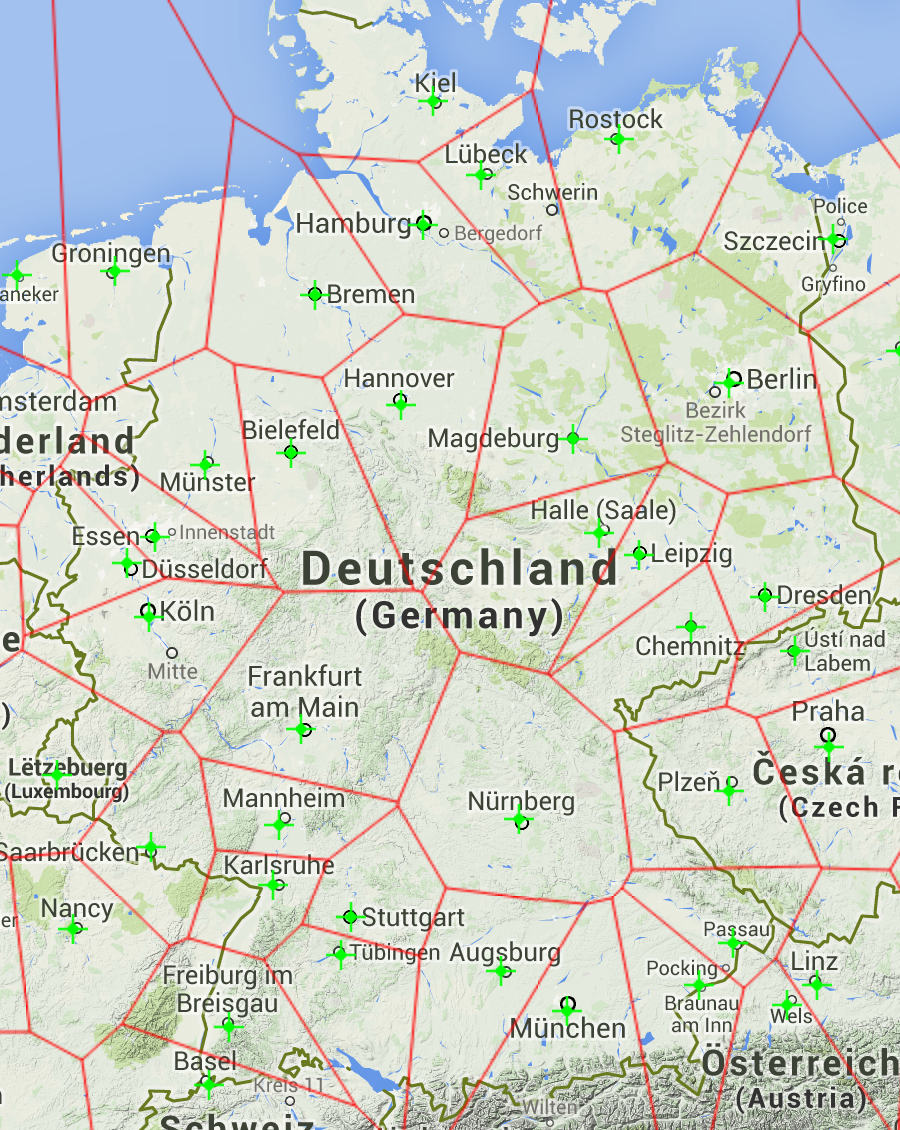
\includegraphics[scale=0.5]{voronoi.png}
				\caption{Beispiel eines Voronoi-Diagramm für einige deutsche Städte}
				\label{img:voronoi}
				\end{center}
			\end{figure}	

			% Quelle: http://lpetrich.org/Science/GeometryDemo/GeometryDemo_GMap.html

			In dicht besiedelten Gebieten können viele kleine Städte vorhanden sein. 
			Damit wäre die Positionsangabe wiederum zu genau.
			Es werden deshalb nur Städte verwendet, deren Einwohnerzahl 15000 überschreitet.
			Jeder Referenzwert wird also der nächstgelegenen Stadt mit mehr als 15000 Einwohnern zugeordnet.
			In Ballungsräumen sind damit mehr Städte zu erwarten, womit kleinere Voronoi-Regionen entstehen.
			Dadurch nimmt die Genauigkeit zu.
			In diesen Gegenden sind allerdings auch mehr Tweets zu erwarten, womit pro Voronoi-Region für die spätere Auswertung ausreichend Referenzwerte vorhanden sind. 
			In ländlichen Gebieten sind hingegen viele kleine Orte und nur wenigen große Städte zu erwarten. 
			Diese werden dadurch in größere Voronoi-Regionen eingeteilt.
			Es sind allerdings auch weniger Tweets zu erwarten. 
			Durch das größere Einzugsgebiet kann dennoch eine ausreichende Anzahl an Referenzwerten einer Stadt zugeordnet werden. 

			Die geografischen Koordinaten der Referenzwerte werden dadurch auf eine definierte Menge geografischer Koordinaten abgebildet. 
			Jeder dieser geografischen Koordinaten ist eine Stadt zugeordnet.
			Dies kann als Übergang einer kontinuierlichen Darstellung durch geografische Koordinaten zu einer diskreten Darstellung durch Städte angesehen werden. 
			Durch die Teilmengenbeziehung ist es nun nicht mehr nötig, die geografischen Regionen der anderen Hierarchieebenen zu bestimmen. 
			Diese werden durch die Stadt implizit mitbestimmt.
			
			\textit{Bewertung des Verfahrens zur Bestimmung der nächstgelegenen Stadt}

				Die Auflösung der geografischen Koordinaten auf Städte wurde mit Hilfe des Ortsverzeichnisses geonames.org umgesetzt.
				Jeder Stadt ist dabei eine geografische Koordinate zugeordnet.
				Wird nach obigem Verfahren eine geografische Position auf eine Stadt aufgelöst, entstehen Ungenauigkeiten.
				Um das Verfahren zu bewerten, wurden die Distanzen, welche zwischen der tatsächlichen Position eines Tweets und der zugeordneten Position der Stadt liegen, protokolliert. 
				Dies spiegelt den Fehler des Zuordnungsverfahrens wieder.

				In Tabelle \ref{tab:distances} sind die Ergebnisse dargestellt.
				Es wurden 383222 Tweets untersucht.
				Im Median liegt die Fehlerdistanz zwischen der tatsächlichen Position und der zugeordneten Stadt bei 3,5 Kilometern.
				Über die Quantile können die Fehlerdistanzen noch genauer untersucht werden.
				Das 0.25 Quantil sagt aus, dass 25\% aller Fehlerdistanzen unter 1,7 Kilometern liegen.
				Der Wert für das 0.95 Quantil liegt bei 24,1 Kilometer, 95\% der Tweets waren näher als 24,1 Kilometer an der zugeordneten Stadt. 
				
				Es wird dadurch auch deutlich, dass ein Großteil der Tweets in der Nähe größerer Städte abgesendet wurden. 
				95\% der Tweets wurden im Abstand von weniger als 24 Kilometern zu einer Stadt mit mehr als 15000 Einwohnern versendet.

					\begin{table}[h]
					\centering
					\caption{Fehlerdistanzen zwischen Tweet Ursprung und zugeordneter Stadt (in km)}
					\label{tab:distances}
					\begin{tabular}{|l|l|}
					\hline
					Durchschnitt & 7      \\ \hline
					Median       & 3.5    \\ \hline
					0.25 Quantil & 1.7    \\ \hline
					0.75 Quantil & 6.9    \\ \hline
					0.85 Quantil & 10     \\ \hline
					0.95 Quantil & 24.1   \\ \hline
					0.98 Quantil & 44.2   \\ \hline
					Größte Distanz      & 3424.5 \\ \hline
					Kleinste Distanz     & 0     \\ \hline
					\end{tabular}
					\end{table}

			\textit{Grenzen des Verfahrens zur Bestimmung der nächstgelegenen Stadt}

				Es ist zu beachten, dass durch die Erzeugung der Voronoi-Regionen Ländergrenzen nur approximiert werden können. 
				Voronoi-Regionen zu Städten die in der Nähe einer Landesgrenze liegen können über die Landesgrenzen hinausgehen. 
				Damit werden geografische Positionen unter Umständen dem falschen Land zugeordnet.
				Auch dies ist in Abbildung \ref{img:voronoi} an den Landesgrenzen zu erkennen. 
				Umso größer allerdings die Anzahl der Städte ist die betrachtet wird, umso genauer wird die Approximation. 

		\section{Zusammenfassung und Beispiel}

			Es wurden die Werte im Nutzer-Standortfeld durch die in den Abschnitten \ref{sub:Vorv}, \ref{sub:VorvNGramme} und \ref{sub:VorvNutzerZeitzone} vorgestellten Schritte verarbeitet.
			Es entsteht dadurch eine Menge von Referenzwerten.
			
			Mit Hilfe der geografischen Koordinaten wird jeder Referenzwert der nächstgelegenen Stadt zugeordnet (siehe Abschnitt \ref{sub:Stadtbestimmen}). 
			
			In einem letzten Schritt werden, basierend auf diesen Ergebnissen, die Vorkommen der Referenzwerte pro geografischer Position aufsummiert.
			Diese Referenzwerte werden in der Georeferenz-Basis gespeichert.

			In Abbildung \ref{img:bspEinlernen} ist das Einlernen an einem Beispiel dargestellt.
			Auf der linken Seite sind 5 Lerndatensätze dargestellt.
			Dabei ist NSt der Nutzer-Standort, NZz die Nutzer-Zeitzone und GKo sind die geografischen Koordinaten.
			
			Diese Werte werden in eine Menge Referenzwerte überführt.
			Zudem wird jedem Referenzwert die nächstgelegene Stadt zugeordnet.
			Dies wird durch die Pfeile zwischen den Lerndatensätzen und dem Mittelblock dargestellt.
			
			Die Pfeile vom Mittelblock auf die Georeferenz-Basis zeigen an, welche Datensätze übereinstimmen und deshalb zusammengefasst werden. 
			
			Die restlichen Datensätze werden direkt in die Georeferenz-Basis übertragen und die absolute Häufigkeit wird mit 1 initialisiert. \footnote{Die Pfeile beim direkten Eintragen wurden ausgelassen, um das Diagramm übersichtlich zu halten.} 
			
			In diesem Beispiel wird deutlich wie durch die Verarbeitung einige Probleme bei der Verwendung des Nutzer-Standortes vermieden werden.

			Datensatz 1 besitzt nur partiellen geografischen Bezug (siehe Abschnitt \ref{sub:partiellerGeografischerBezug}). 
			Trotzdem kann durch die Zerlegung der Wert "'New+York"', der ein Toponym darstellt, genutzt werden.
			Damit entsteht ein Eintrag in der Georeferenz-Basis für die Kombination "'New+York"' und New York City (NYC).

			Die Werte in Datensatz 2 stellen eine Hierarchiebeziehung dar.
			Diese Hierarchie bleibt durch ein Bi-Gramm erhalten.
			Trotzdem kann die absolute Häufigkeit für die Kombination "'New+York"' und NYC inkrementiert werden, da "'New+York"' durch die Uni-Gramme auch separat betrachtet werden kann.
			Es wurde also durch die separate Betrachtung eine zusätzliche Information extrahiert.

			Datensatz 3 und 5 weisen eine Doppeldeutigkeit auf.
			Die geografischen Koordinaten von Datensatz 3 werden auf York in Großbritannien (YO(GB)) aufgelöst.
			
			Datensatz 4 wird hingegen York in den USA als Georeferenz zugeordnet (YO(US)). 
			Allein durch die Betrachtung des Uni-Grammes "'York"' können die beiden Städte nicht unterschieden werden. 
			Bezieht man jedoch die Nutzer-Zeitzone ein können die Werte unterschieden werden. 

			Datensatz 4 weist einen Widerspruch im Nutzer-Standort auf (siehe Abschnitt \ref{sub:wiederspruechlicheBezuege}). 
			Durch die Auflösung der geografischen Koordinaten auf eine Stadt und die Möglichkeit, die Werte als Uni-Gramme einzeln zu betrachten kann dennoch eine Information daraus gewonnen werden. 
			
			Im Beispiel werden die geografischen Koordinaten auf die Stadt York in Großbritannien aufgelöst.
			Auch das Toponym "'York"' taucht im Nutzer-Standort auf und wird deshalb der Stadt York zugeordnet.  
			Durch Datensatz 3 ist diese Kombination schon in der Georeferenz-Basis vorhanden und es wird die absolute Häufigkeit inkrementiert.
			Gleiches gilt für den Referenzwert bestehend aus Uni-Gramm und Nutzer-Zeitzone.
			
			Das bedeutet, selbst wenn widersprüchliche Werte angegeben sind, kann eine gewinnbringende Information aus dem Datensatz gezogen werden.

			Durch diese Verarbeitung entstehen auch Datensätze in der Georeferenz-Basis, die nur einmal vorkommen.
			Diese sollen allerdings nicht verworfen werden. 
			Es wird dadurch in der Geolokalisierung ermöglicht, tiefer gehende Analysen der Vorkommen von Referenzwerten durchzuführen. 

			\begin{figure}[H]
				\begin{center}
				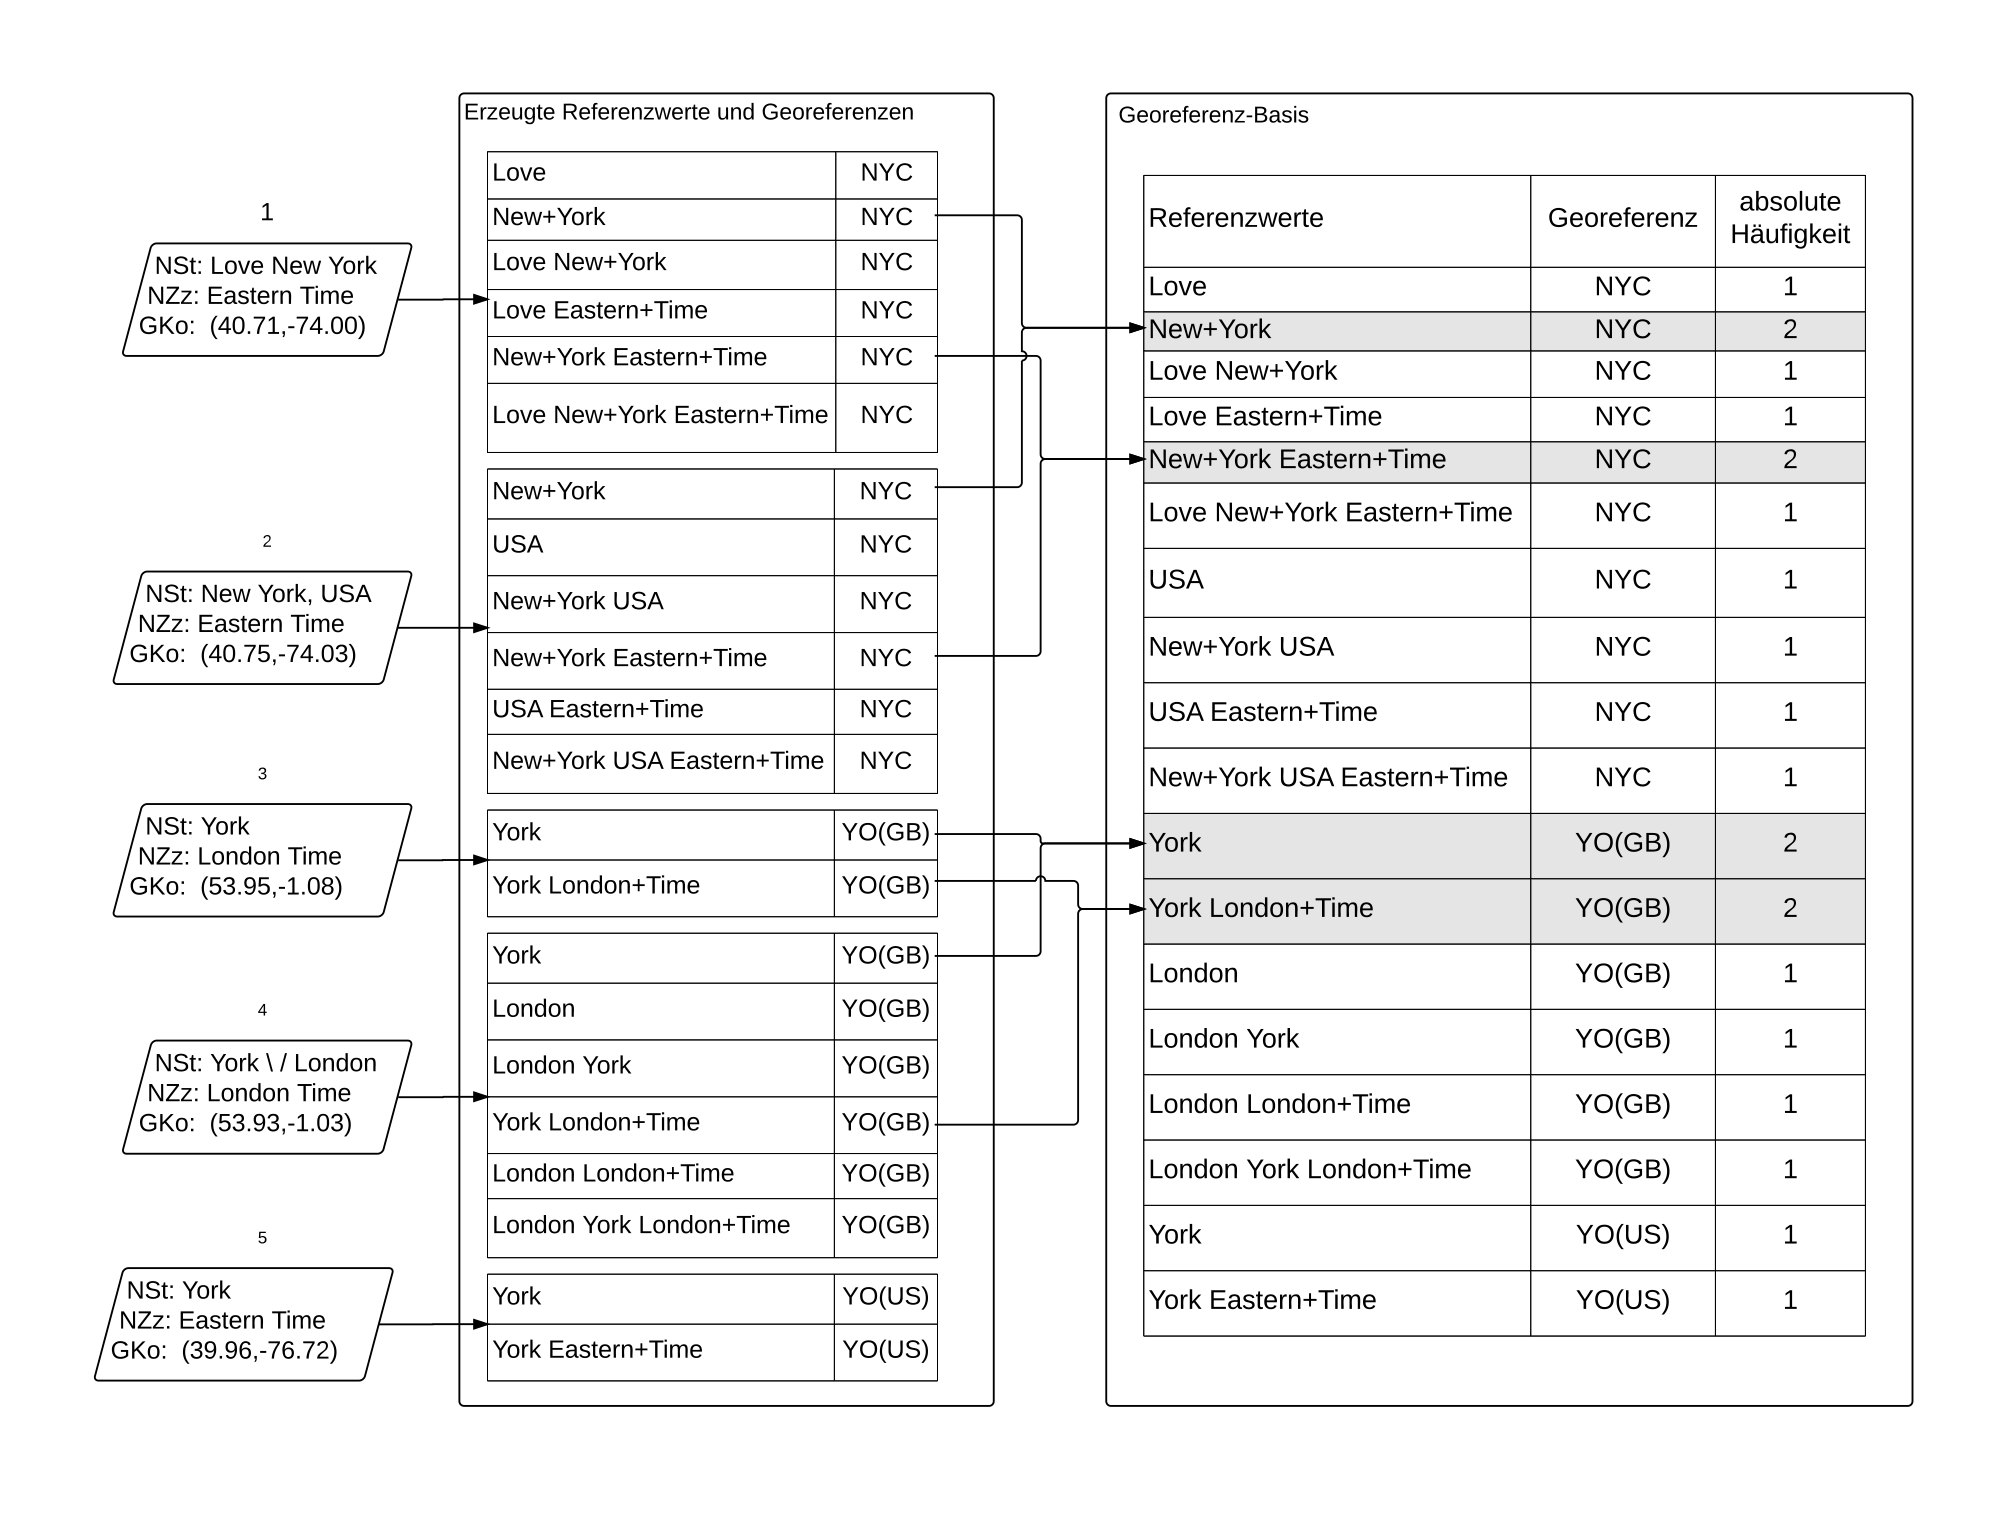
\includegraphics[scale=0.4]{bspEinlernen.png}
				\caption{Beispiel: Einlernen der Georeferenz-Basis}
				\label{img:bspEinlernen}
				\end{center}
			\end{figure}	
				

	\section{Geolokalisierung: Auflösen des Nutzer-Standortes mit Hilfe der Georeferenz-Basis} \label{sec:AufloesenDesNutzerStandortes} 

		Es wird nun das Verfahren zur Geolokalisierung eines Tweets vorgestellt.
		Dabei dient die Georeferenz-Basis und die in ihr abgelegten Referenzwerte als Basis für die Zuweisung einer Georeferenz.

		In Abbildung \ref{img:ablaufGeolok} ist der gesamte Ablauf der Geolokalisierung dargestellt.
		Aus dem Nutzer-Standortfeld und der Nutzer-Zeitzone werden zunächst potenzielle geografische Indikatoren erzeugt.
		Dies geschieht analog zur Erzeugung von Referenzwerten beim Einlernen der Georeferenz-Basis.
		Es werden dazu die Schritte aus den Abschnitten \ref{sub:Vorv}, \ref{sub:VorvNGramme} und \ref{sub:VorvNutzerZeitzone} diese Schritte werden in diesem Abschnitt als Vorverarbeitung bezeichnet.
		
		Daraus resultiert eine Menge potenzieller geografischer Indikatoren.
		
		Die Werte der potenziellen geografischen Indikatoren werden nun in der Georeferenz-Basis nachgeschlagen. 
		Dabei werden alle Datensätze, deren Referenzwerte mit den potenziellen geografischen Indikatoren korrespondieren, zurückgegeben.
		
		Basierend auf diesen Datensätzen erfolgt in einem Analyse-Schritt die Bestimmung der Georeferenz.

			\begin{figure} 
			\begin{center}
						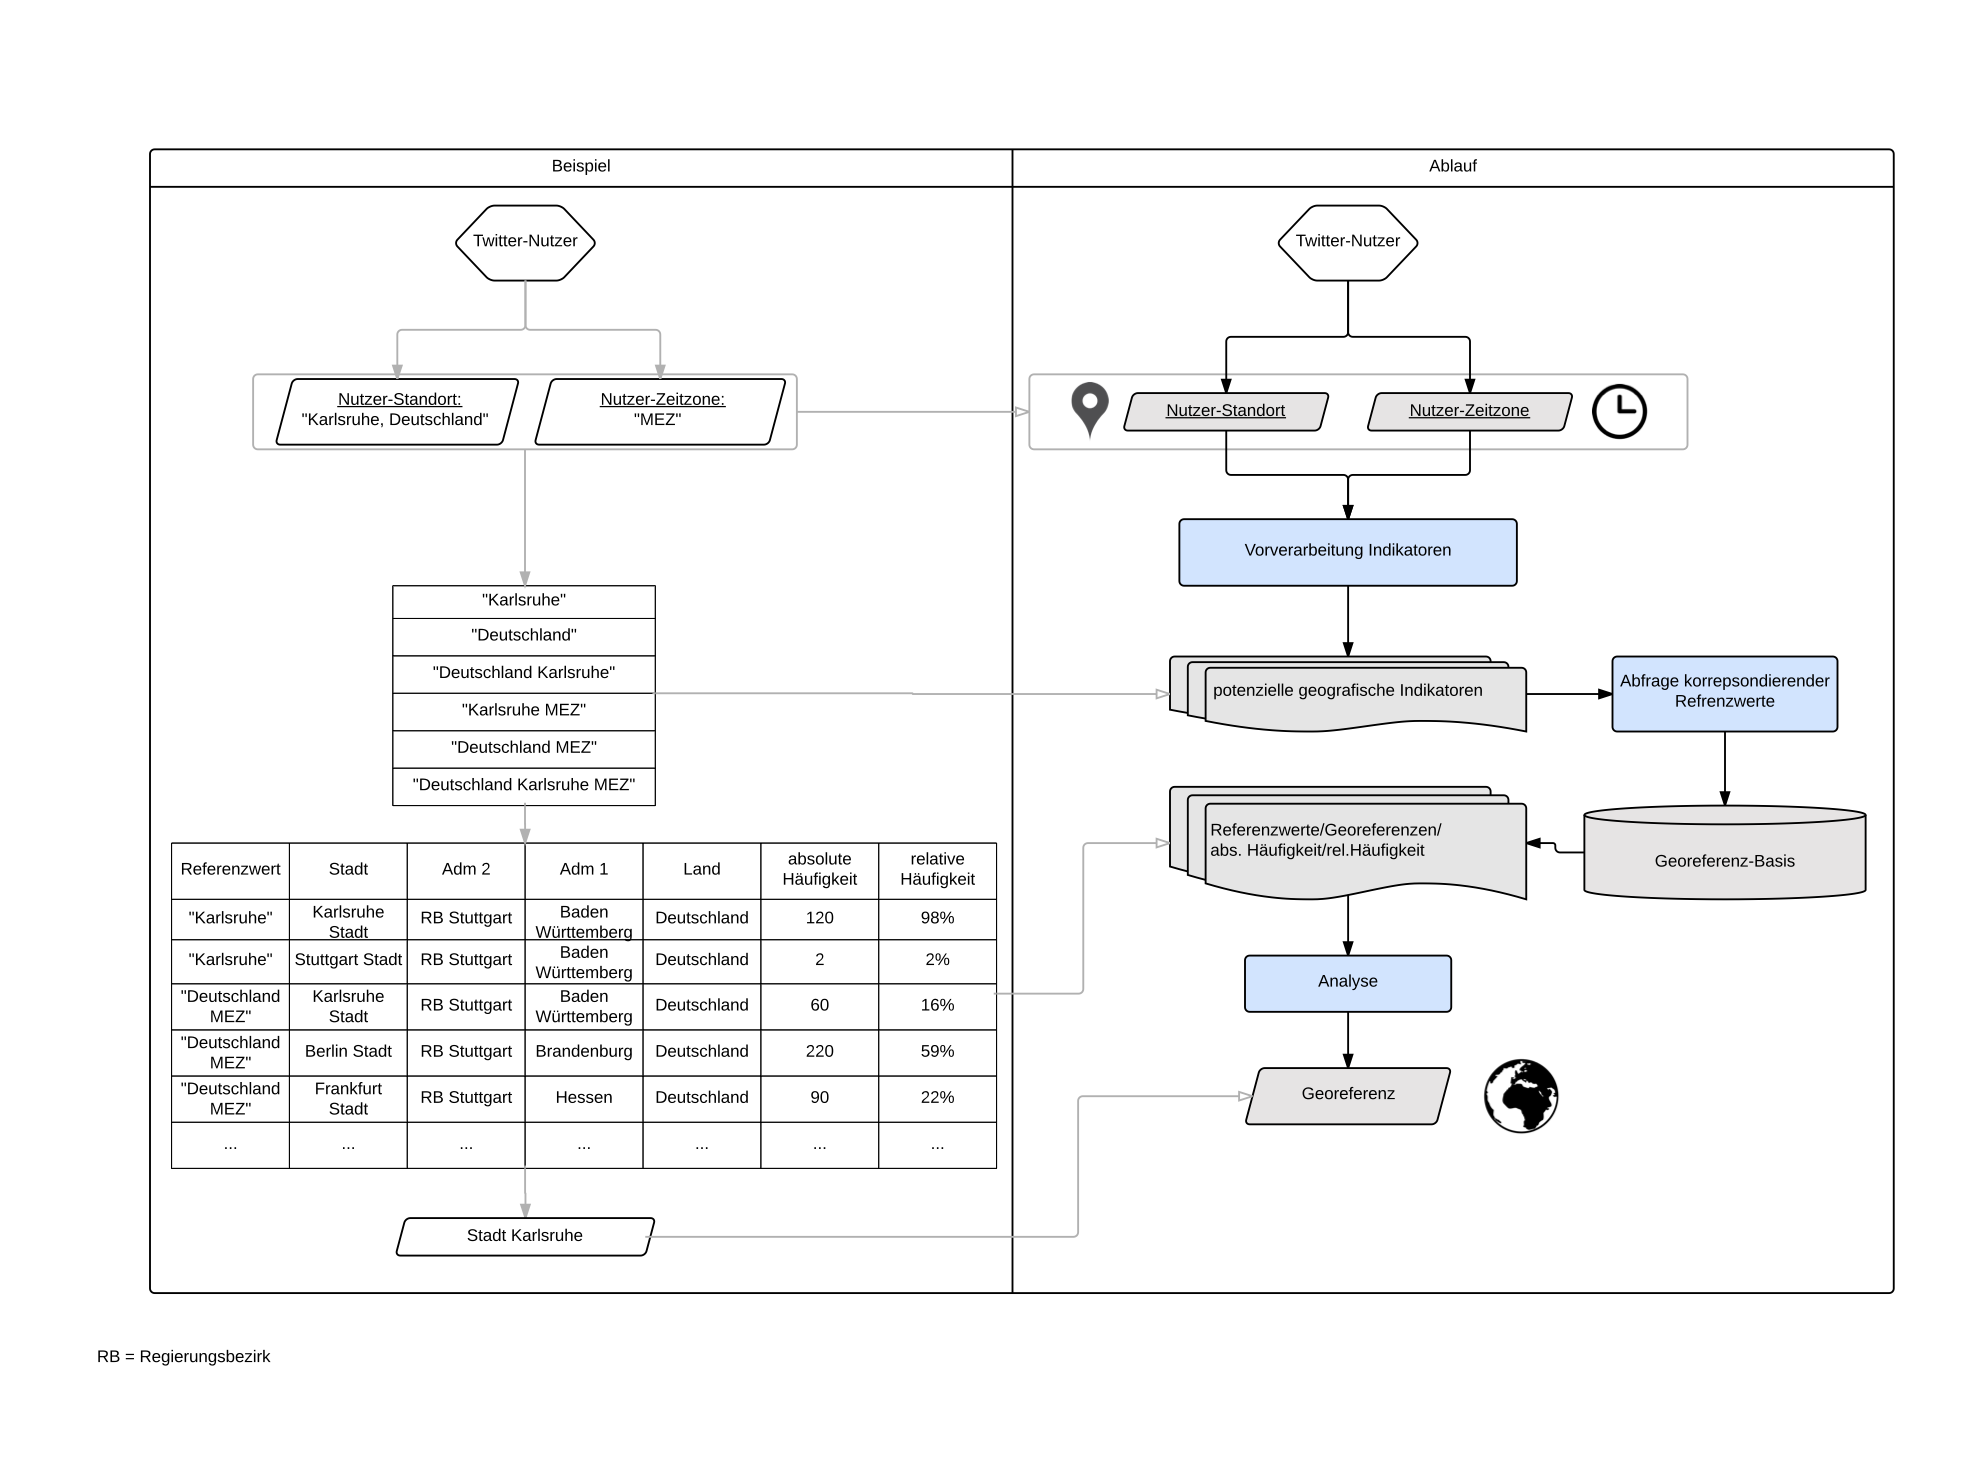
\includegraphics[scale=0.5]{geolokalisierungAllg.png}
						\caption{Ablauf der Geolokalisierung mit Beispiel}
						\label{img:ablaufGeolok}
					\end{center}
			\end{figure}	

		Das zentrale Element der Geolokalisierung ist der Analyse-Schritt. 
		Das Ziel des Analyse-Schrittes ist es, eine Georeferenz zu ermitteln.
	
		Beim Einlernen wurden keine Informationen verworfen, da noch keine Entscheidung über deren geografischen Bezug getroffen werden konnte.
		In der Georeferenz-Basis sind alle Werte enthalten, die aus den Nutzer-Standorten der Lerndatensätze beim Einlernen erzeugt wurden.
		Es sind also auch Referenzwerte vorhanden, die keinen geografischen Bezug aufweisen.
		
		Wird einem potenziellen geografischen Indikator durch einen Referenzwert ohne geografischen Bezug eine Georeferenz zugewiesen, ist diese mit hoher Wahrscheinlichkeit fehlerhaft.
		Dies wiederum führt zu schlechten und unzuverlässigen Ergebnissen.

		Durch den Analyse-Schritt soll nun folgende Frage beantwortet werden: 
		\\ Wie kann bestimmt werden, ob ein Referenzwert geografischen Bezug hat oder nicht? \\
		Oder anders ausgedrückt: 
		\\ Wie kann vermieden werden, dass ein Referenzwert, der keinen geografischen Bezug hat, zur Geolokalisierung genutzt wird?

		Es wird nun kurz auf die Vorverarbeitung des Nutzer-Standortfeldes eingegangen.
		Danach wird ausschließlich der Analyse-Schritt des Verfahrens betrachtet.

		\subsection{Vorverarbeitung des Nutzer-Standortfeldes (Geolokalisierung)}

			Die Schritte der Vorverarbeitung wurden bereits in den Abschnitten \ref{sub:Vorv}, \ref{sub:VorvNGramme} und \ref{sub:VorvNutzerZeitzone} behandelt. 
			Bei der Geolokalisierung werden diese Schritte ebenfalls auf das Nutzer-Standortfeld angewendet.
			Dadurch entstehen folgende Vorteile:

			Sind die Werte in einem Nutzer-Standortfeld gleich wie diejenigen eines bereits eingelernten Nutzer-Standortfeldes, werden bei der Abfrage an die Georeferenz-Basis genau diese Werte zurückgeliefert.

			Die Werte werden angeglichen. 
			Das heißt etwaige Sonder- und Satzzeichen und die Reihenfolge werden beim Vergleichen der Referenzwerte mit den potenziellen geografischen Indikatoren keine Rolle spielen.
			
			Nutzer-Standortfelder mit partiellem geografischen Bezug können besser untersucht werden, da die Werte durch die N-Gramme einzeln abgefragt werden.

			Lediglich das Problem, dass in einem Nutzer-Standortfeld widersprüchliche Angaben gemacht werden, kann zu einem Problem führen. 
			Ohne die Nutzer-Zeitzone kann nicht entschieden werden, welcher Wert genutzt wird.
			Lediglich durch Einbeziehen der Nutzer-Zeitzone besteht eine Chance, die korrekte Georeferenz zu wählen.
			Dies setzt allerdings voraus, dass die beiden angegebenen geografischen Objekte in zwei unterschiedlichen Zeitzonen liegen.

			Ist eine geografische Hierarchieebene angegeben bleibt diese erhalten.
			Durch die alphanumerische Sortierung spielt auch die Reihenfolge der Werte keine Rolle.

			Doppel- und Mehrdeutigkeiten können durch die Nutzer-Zeitzone aufgelöst werden. 
			
		\subsection{Analyse auf Basis absoluter Häufigkeiten} 

			In der Georeferenz-Basis sind die absoluten Häufigkeiten hinterlegt.
			Diese sagen aus wie oft ein Referenzwert in der Voronoi-Region einer Stadt aufgetreten ist (siehe Abschnitt \ref{sub:absHaufBestimmen}). 
			Aus der absoluten Häufigkeit kann abgeleitet werden, ob ein Referenzwert geografischen Bezug hat oder nicht.

			Eine hohe absolute Häufigkeit in einer Voronoi-Region kann ein Hinweis auf den geografischen Bezug eines Referenzwertes zu dieser Region darstellen. 
			Es ist beispielsweise anzunehmen, dass in der Voronoi-Region einer Stadt der Name der zugehörigen Stadt häufig vorkommt.

			In Abbildung \ref{img:ulIstanbulWalesZoom} sind die Tweets in denen "'Istanbul"' im Nutzer-Standort vorkommt aufgetragen.
			Es tritt deutlich eine Konzentrierung um die Stadt Istanbul auf. 
			Diese Tweets werden auf die Stadt Istanbul abgebildet.
			An dieser geografischen Position wird die Kombination aus dem Referenzwert "'Istanbul"' und der Georeferenz Istanbul sehr häufig vorkommen.
			In den Nutzer-Standorten der Tweets rund um Istanbul taucht "'Istanbul"' tatsächlich 972 mal auf.
			Damit kann eine Relevanz für den Referenzwert "'Istanbul"' zur Stadt Istanbul abgeleitet werden.

			\begin{figure}[!ht]
					\centering
						\makebox[\textwidth]{
						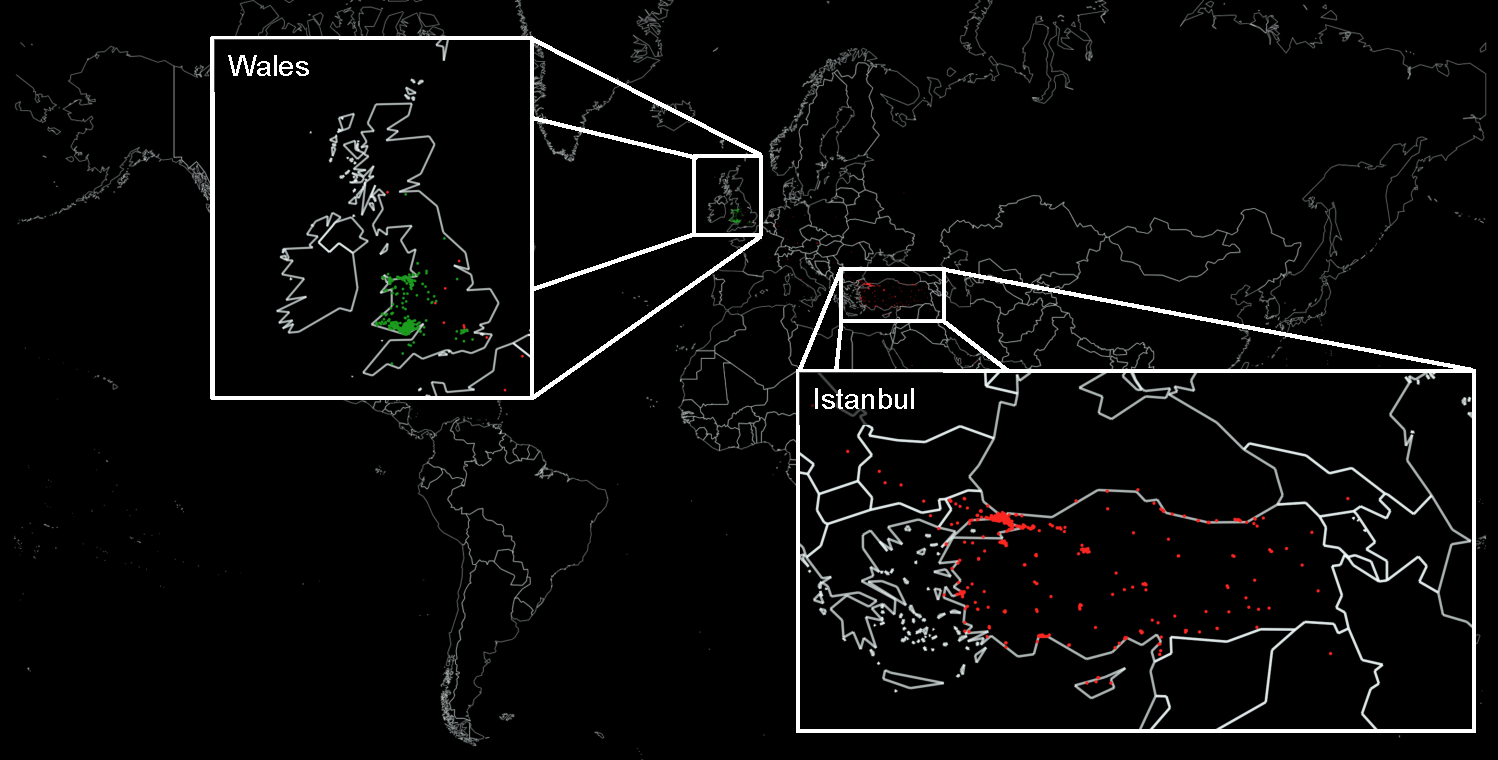
\includegraphics[scale=0.7]{ulIstanbulWalesZoom.pdf}
						} 
						\caption{Verteilung der Tweets die "'Istanbul"' (rot) oder "'Wales"'' (grün) im Nutzer-Standortfeld enthalten}
						\label{img:ulIstanbulWalesZoom}


			\end{figure}	


			\subsubsection{Schwellwert für die absolute Häufigkeit} 

				Um Referenzwerte mit geografischem Bezug zu identifizieren, wird ein Schwellwert für die absolute Häufigkeit eingeführt.
				Es werden nur Referenzwerte zur Geolokalisierung verwendet, deren absolute Häufigkeit über diesem Schwellwert liegt.
				Je höher der Schwellwert gewählt wird, umso häufiger muss ein Referenzwert in einer Voronoi-Region vorgekommen sein, um in Betracht gezogen zu werden.
				Dadurch steigt die Wahrscheinlichkeit, dass der zugehörige Referenzwert geografischen Bezug hat. 
				Durch den Schwellwert wird es zudem ermöglicht, die Güte und die Trefferquote zu beeinflussen.
				Umso geringer der Schwellwert gewählt wird, umso mehr Referenzwerte können in die Betrachtung einbezogen werden, allerdings ist die Wahrscheinlichkeit, dass diese geografischen Bezug aufweisen geringer.  

			\subsubsection{Ablauf}

				Für jeden potenziellen geografischen Indikator wird aus den Ergebnisdatensätzen derjenige Datensatz gewählt, der die größte absoluten Häufigkeit über dem Schwellwert aufweist.
				Aus diesen Datensätzen wird wiederum derjenige mit der größten absoluten Häufigkeit gewählt. 
				Das Ergebnis ist ein einzelner Datensatz, dessen Georeferenz dem untersuchten Tweet zugewiesen wird.

				In Abbildung \ref{img:absHaufBsp} wird der Ablauf dargestellt.
				Der Schwellwert wurde dabei auf 10 Vorkommen in einer Voronoi-Region festgelegt. 
				
				\begin{figure}[!ht]
	
						\centering
						\makebox[\textwidth]{
						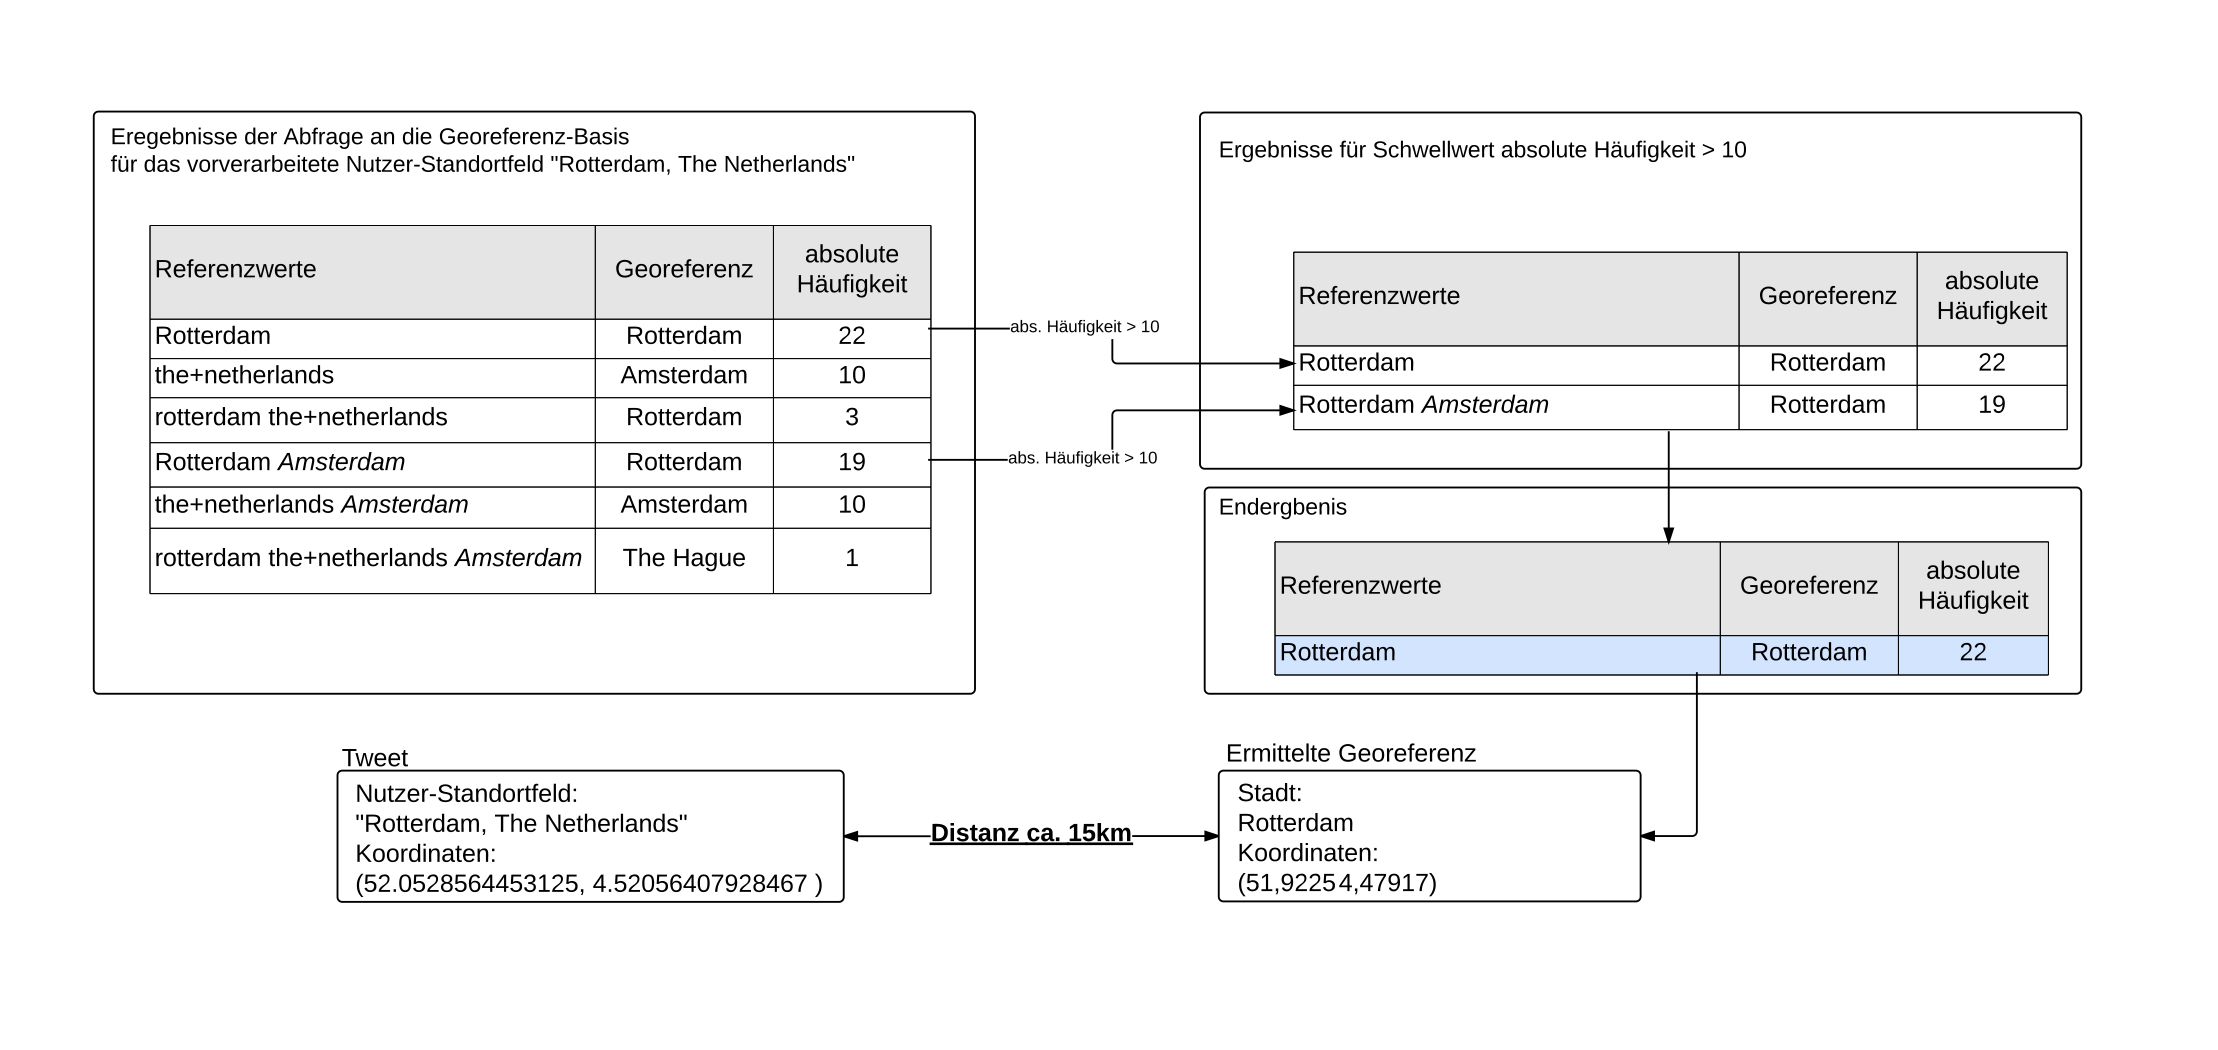
\includegraphics[scale=0.4]{absHaufBsp.png} 
						} 
						\caption{Ablauf: Analyse basierend auf absoluten Häufigkeiten}
						\label{img:absHaufBsp}
					
				\end{figure}

		\subsubsection{Probleme bei der ausschließlichen Betrachtung der absoluten Häufigkeiten} 

			Bei der Analyse basierend auf absoluten Häufigkeiten wird die Verteilung des Referenzwertes auf dem Globus nicht berücksichtigt.
			Ein Referenzwert kann eine gleichmäßige Verteilung über den Globus aufweisen.
			Das bedeutet, der Referenzwert wird an vielen unterschiedlichen Orten benutzt. 
			Wörter wie das englische Wort "'in"' können in einer Voronoi-Region dennoch sehr häufig auftreten. 
			Es ist aber nicht davon auszugehen, dass "'in"' einen geografischen Bezug hat.  
			Der Wert der absoluten Häufigkeiten kann für solche Wörter sogar über einem gewählten Schwellwert liegen.
			Die Häufung kann jedoch relativ, im Vergleich zur globalen Verwendung, sehr gering sein.
			Dies ist ein Hinweis darauf, dass der Referenzwert keinen geografischen Bezug hat.
			Über die relative Häufigkeit kann die Verteilung des Referenzwertes bestimmt werden. 
			Es ist also wichtig nicht nur die absoluten Häufigkeiten, sondern auch die relativen Häufigkeiten, und damit die globale Verteilung der Referenzwerte zu berücksichtigen.

			Dies soll anhand eines Beispiels verdeutlicht werden.
			In Argentinien liegt die Stadt La Plata. 
			Ein Referenzwert "'La Plata"' hat also offensichtlich geografischen Bezug.
			"'La Plata"' tritt tatsächlich in der Voronoi-Region der Stadt La Plata 91 mal auf (siehe Tabelle \ref{tab:laPlataAbs}).			 
			Betrachtet man die absoluten Häufigkeiten für den Referenzwert "'La Plata"' könnte man den Schwellwert beispielsweise auf 90 ansetzen.

			\begin{table}[h]
				\centering
				\caption{"'La Plata"'}
				\label{tab:laPlataAbs}
				\begin{tabular}{|l|l|}
				\hline
				Stadt            & abs. Häufigkeit  \\ \hline \hline
				La Plata         & 91              \\ \hline
				Villa Gesell     & 9               \\ \hline
				Mar del Plata    & 5               \\ \hline
				Quilmes          & 3               \\ \hline
				... & ... \\ \hline
				\end{tabular}
			\end{table}

			Der Referenzwert "'the"' hat hingegen keinen geografischen Bezug.
			Trotzdem tritt der Wert 91 mal in der Stadt Jakarta auf (siehe Tabelle \ref{tab:theAbs}). 
			Mit einem Schwellwert von 90, für die absolute Häufigkeit, würde dem Referenzwert "'the"' ein geografischer Bezug attestiert.
			Betrachtet man allerdings Abbildung \ref{img:ULThe} fällt auf, dass Tweets mit dem Wert "'the"' im Nutzer-Standort sehr verteilt auf dem Globus auftreten.
			Wird ein Tweet mit dem Wert "'the"' im Nutzer-Standortfeld geolokalisiert wird diesem mit hoher Wahrscheinlichkeit eine falsche Georeferenz zugewiesen.

			Im Gegensatz dazu tritt "'La Plata"' in den Nutzer-Standorten sehr konzentriert auf (siehe Abbildung \ref{img:ULlaPlata}).
			Es ist deutlich eine Häufung um die Stadt La Plata in Argentien zu erkennen, weltweit tritt der Referenzwert aber sehr selten auf.

			\begin{table}[h]
				\centering
				\caption{"'the"'}
				\label{tab:theAbs}
				\begin{tabular}{|l|l|}
				\hline
				Stadt             & abs. Häufigkeit \\ \hline \hline
				Jakarta           & 91              \\ \hline
				Singapore         & 27              \\ \hline
				Bekasi            & 25              \\ \hline
				Philadelphia      & 23              \\ \hline
				... & ... \\ \hline
				\end{tabular}
				\end{table}

			\begin{figure} 
				\begin{center}
					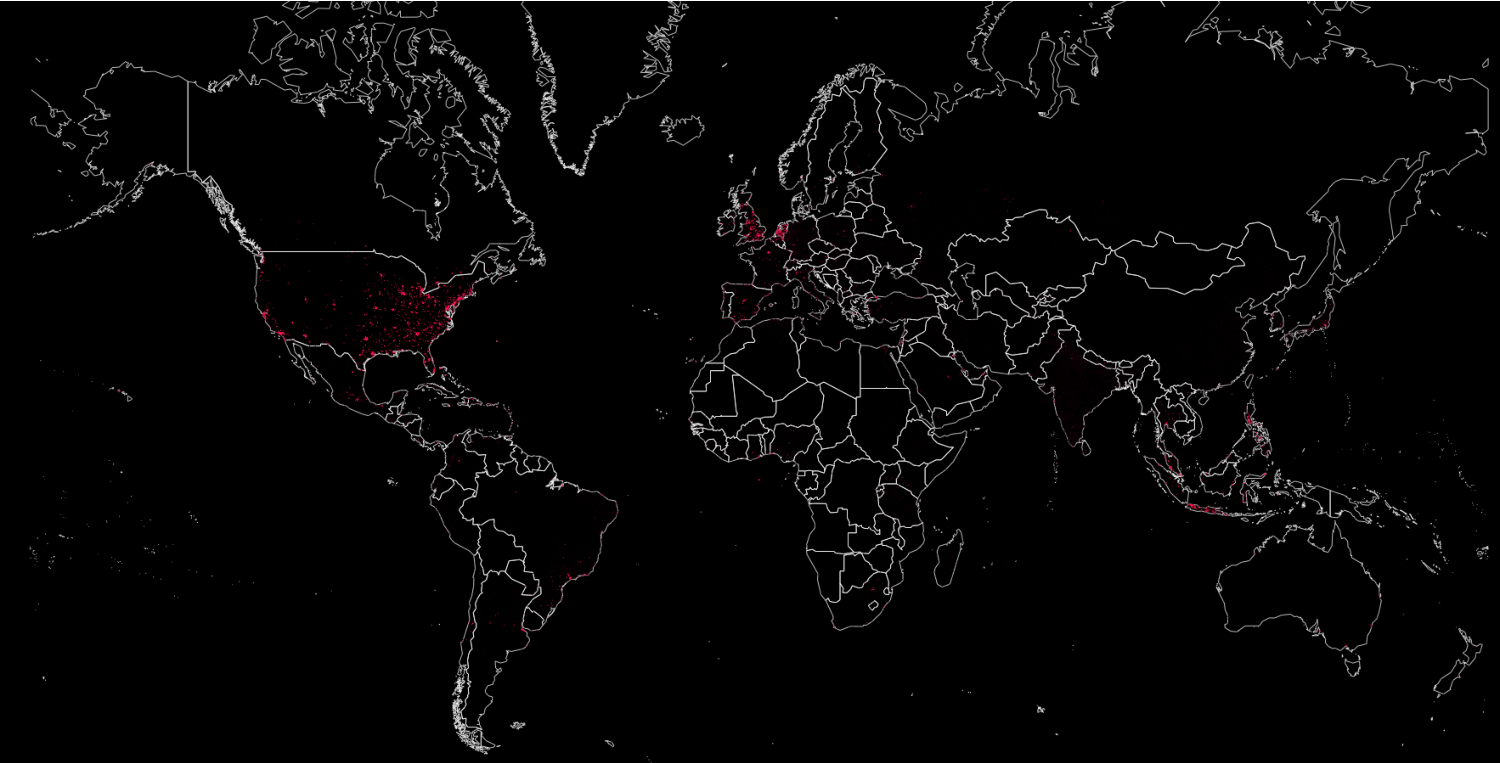
\includegraphics[scale=0.6]{ulTheG.pdf}
					\caption{Tweets in denen im Nutzer-Standort "'the"' auftaucht}
					\label{img:ULThe}
					\end{center}
				\end{figure}
			\begin{figure}

			\begin{center}
					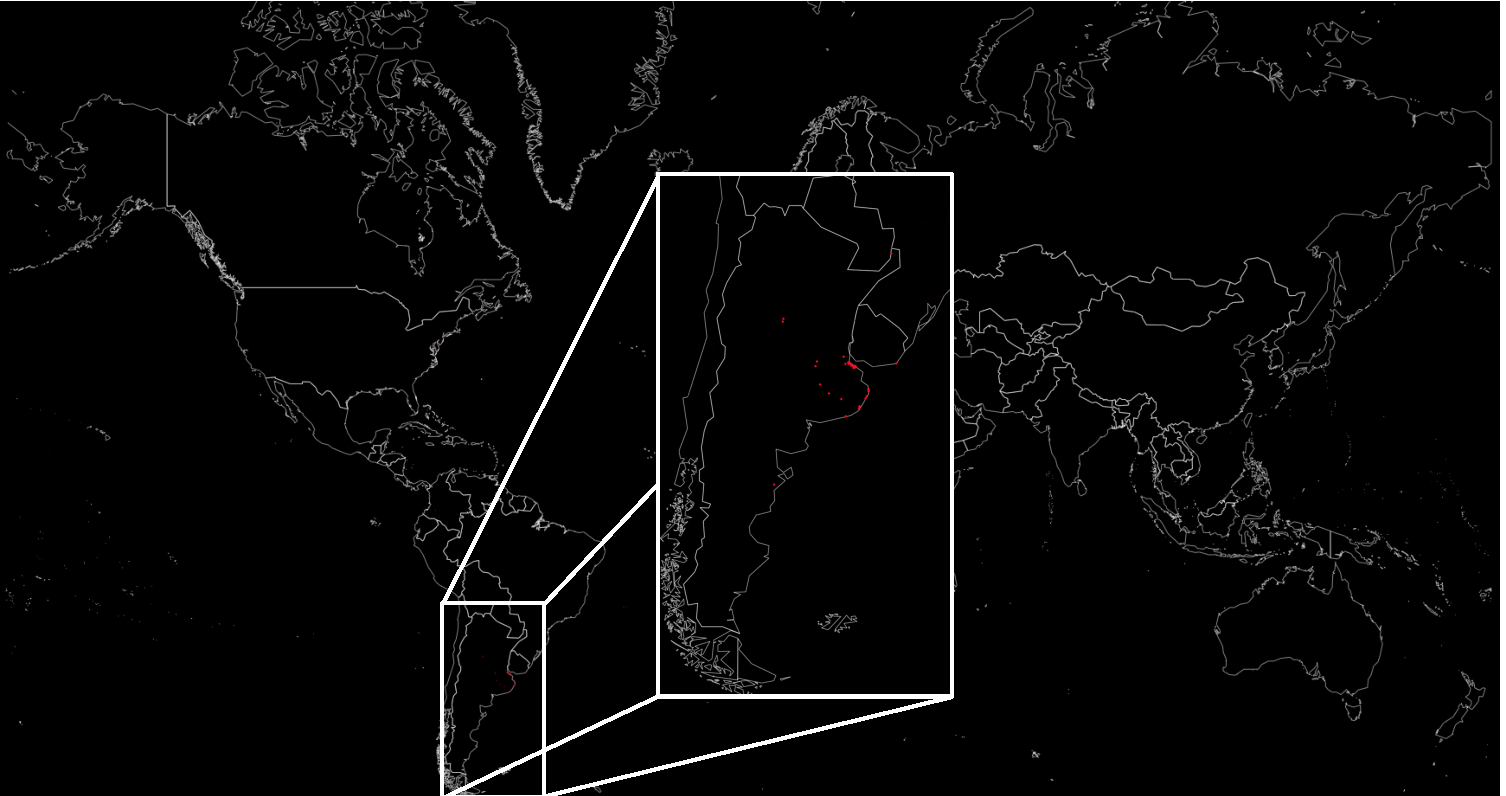
\includegraphics[scale=0.5]{ulLaPlataG.pdf}
					\caption{Tweets in denen im Nutzer-Standort "'La Plata"' auftaucht}
					\label{img:ULlaPlata}
				\end{center}
			\end{figure}	


			Es werden deshalb zusätzlich die relativen Häufigkeiten betrachtet.	

		\subsection{Analyse basierend absoluten und relativen Häufigkeiten} \label{sub:Analyse-absRel} 

			Die Analyse basierend auf absoluten Häufigkeiten ist fehleranfällig. 
			Es wird die Verteilung des Referenzwertes außer acht gelassen.
			Die absolute Häufigkeit gibt lediglich an wie oft ein Wert in einer Voronoi-Region vorkam.
			Die relative Häufigkeit gibt dagegen an welchen Anteil der Gesamtvorkommen auf eine Voronoi-Region entfällt.

			\textit{Berechnung der relativen Häufigkeiten}  

				Um die relativen Häufigkeiten zu berechnen, wird das Vorkommen eines Referenzwertes in einer Stadt, durch die Gesamtanzahl der Vorkommen des Referenzwertes geteilt werden.
				Dies wird mit Hilfe der Georeferenz-Basis realisiert.
				Bei der Abfrage eines potenziellen geografischen Indikators wird nicht nur derjenige Referenzwert mit der größten absoluten Häufigkeit zurückgeliefert, sondern auch die Anzahl der Gesamtvorkommen dieses Referenzwertes.

				Die Funktion $max_{abs}(a)$ liefert die maximale absolute Häufigkeit für einen potenziellen geografischen Indikator $a$ aus der Georeferenz-Basis.
				Die Funktion $sum_{abs}(a)$ liefert die Anzahl der Gesamtvorkommen des potenziellen geografischen Indikators a in der Georeferenz-Basis, dies entspricht der Summe aller absoluten Häufigkeiten aller Vorkommen des Wertes $a$.

				Damit kann die relative Häufigkeit  $rel(a)$ des geografischen Indikators a folgendermaßen berechnet werden.

				\begin{equation}
					rel(a)=\frac{max_{abs}(a)}{sum_{abs}(a)}
				\end{equation}	

			\textit{Betrachtung des Beispiels "'La Plata"' und "'the"' bezüglich relativer Häufigkeiten} 
				
				Bezieht man die relativen Häufigkeiten ein, ergibt sich für den Wert "'the"' Tabelle \ref{tab:the} für "'La Plata"' ergibt sich Tabelle \ref{tab:laPlata}.  

				\begin{table}[h]
				\centering
				\caption{Relative Häufigkeiten für den Referenzwert "'the"'}
				\label{tab:the}
				\begin{tabular}{|l|l|l|}
				\hline
				Stadt             & abs. Häufigkeit & rel. Häufigkeit in \% \\ \hline \hline
				Jakarta           & 91              & 1,6                       \\ \hline
				Singapore         & 27              & 0,5                       \\ \hline
				Bekasi            & 25              & 0,4                       \\ \hline
				Philadelphia      & 23              & 0,4                       \\ \hline
				... & ... & ... \\ \hline
				\end{tabular}
				\end{table}

				\begin{table}[h]
				\centering
				\caption{Relative Häufigkeiten für den Referenzwert "'La Plata"'}
				\label{tab:laPlata}
				\begin{tabular}{|l|l|l|}
				\hline
				Stadt            & abs. Häufigkeit & rel. Häufigkeit in \% \\ \hline \hline
				La Plata         & 91              & 70,5                      \\ \hline
				Villa Gesell     & 9               & 7,0                       \\ \hline
				Mar del Plata    & 5               & 3,9                       \\ \hline
				Quilmes          & 3               & 2,3                       \\ \hline
				... & ... & ... \\ \hline
				\end{tabular}
				\end{table}

				Vergleicht man Tabelle \ref{tab:the} mit Tabelle \ref{tab:laPlata} kann durch die relativen Wahrscheinlichkeiten die globale Verteilung der beiden Werte verglichen werden.
				Es ist deutlich zu erkennen, dass "'La Plata"' (70.5\%) wesentlich konzentrierter auftritt als "'the"' (1,6\%).

			\subsubsection{Schwellwert für die relative Häufigkeit}

				Auch für die relative Häufigkeit wird ein Schwellwert eingeführt. 
				Dieser Schwellwert garantiert, das ein Referenzwert einen bestimmten Anteil an Vorkommen auf eine Voronoi-Region vereint.
				Dadurch können global genutzte Referenzwerte eliminiert werden.
				Der Schwellwert für die absolute Häufigkeit soll allerdings weiterhin verwendet werden. 
				Denn für geringe absolute Häufigkeiten kann die relative Häufigkeit hoch sein.
				Kommt ein Referenzwert in einer Voronoi-Region "'A"' 5 mal vor und in einer Voronoi-Region "'B"' nur ein mal entspricht dies einer relativen Häufigkeit von 83\% für die Voronoi-Region A.
				Trotz der hohen relativen Häufigkeit ist die absolute Häufigkeit gering.    
			
			\subsubsection{Ablauf}

				In Abbildung \ref{img:relHaufBsp} ist der Ablauf der Analyse mit absoluten und relativen Häufigkeiten dargestellt.
				Um den Ablauf übersichtlich zu halten, sind die Referenzwerte mit Zeitzone hier nicht berücksichtigt.
				
				Zuerst werden diejenigen Datensätze verworfen, die unter einem Schwellwert von 5 für die absolute Häufigkeit liegen.
				Danach werden diejenigen Datensätze verworfen, die unter einem Schwellwert von 10\% für die relative Häufigkeit liegen.
				Aus der Restmenge an Datensätzen wird derjenige gewählt, der die größte relative Häufigkeit aufweist. 

				 \begin{figure}[!ht]
	
						\centering
						\makebox[\textwidth]{
						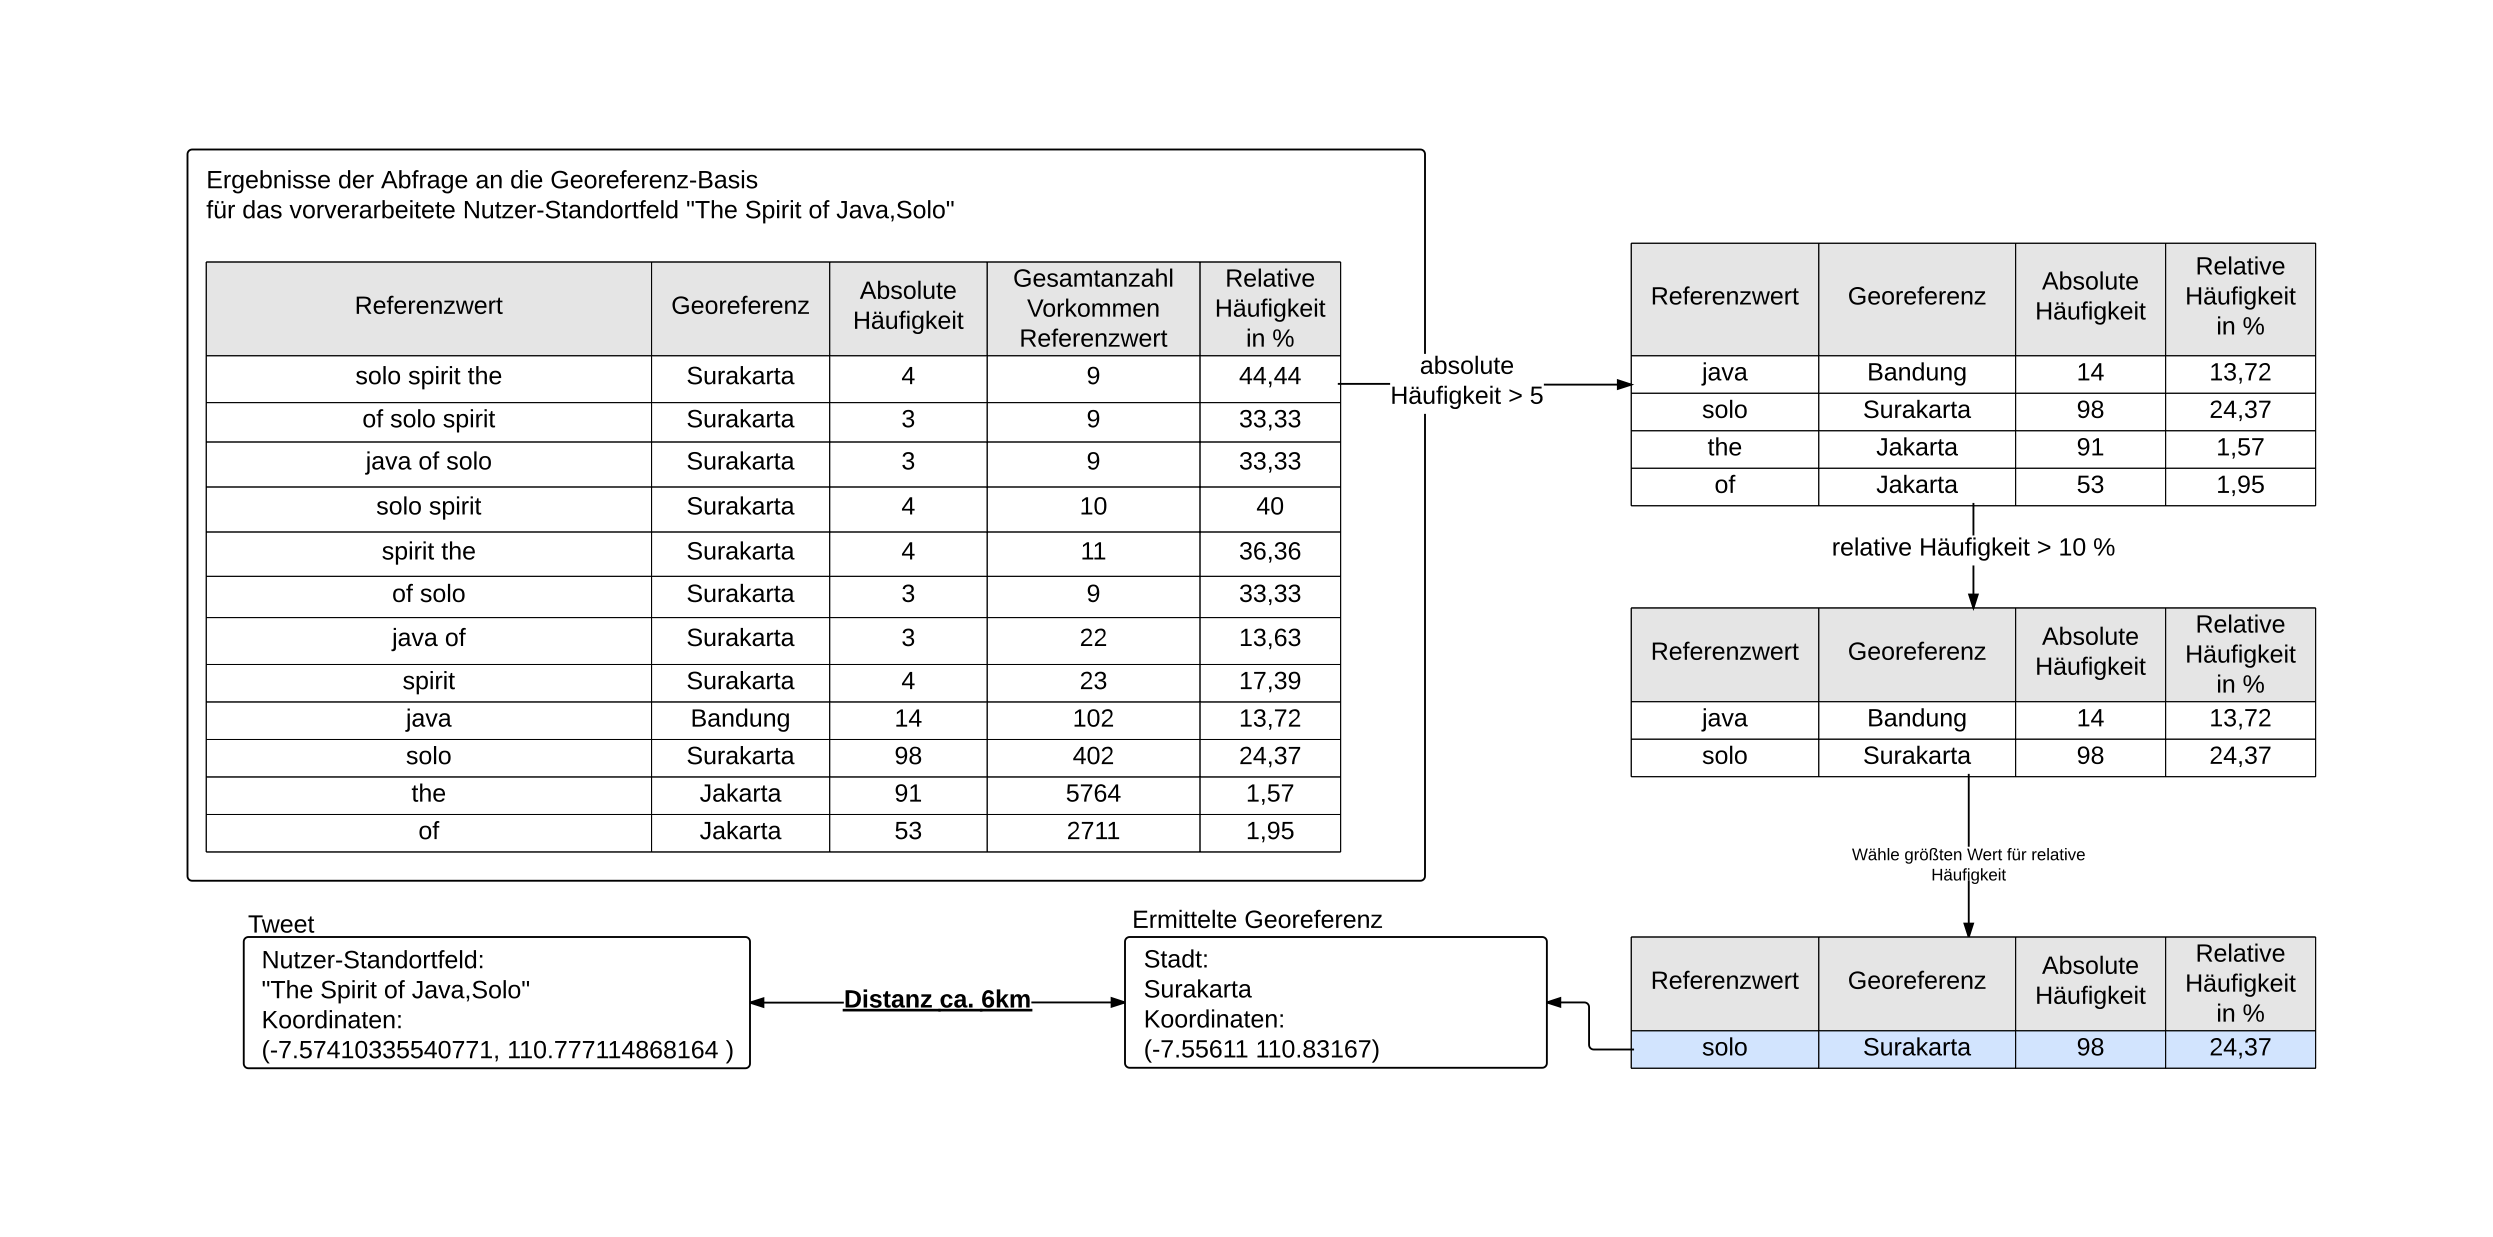
\includegraphics[scale=0.4]{relHaufBsp.png} 
						} 
						\caption{Analyse basierend auf relativen Häufigkeiten}
						\label{img:relHaufBsp}
					
				\end{figure}

				Mit diesem Ablauf wird einerseits garantiert, dass ein Referenzwert oft genug vorkommt und andererseits einen gewissen Anteil am Gesamtvorkommen auf eine Region vereint.

	\section{Verwendung der geografischen Hierarchie} \label{sec:ausnutzenDerGeografischenHierarchie}

		Die geografischen Koordinaten der Tweets werden wie in Abschnitt \ref{img:voronoi} auf die nächstgelegene Stadt aufgelöst. 
		Dies geschieht mit Hilfe des Ortsverzeichnisses geonames.org. 	
		Dieses Ortsverzeichnis bildet die geografische Hierarchieebenen ab (siehe Abschnitt \ref{sub:geografischeHierarchie}). 
		Jeder Stadt werden die Verwaltungseinheiten erster und zweiter Ordnung sowie ein Land zugeordnet.

		Das bedeutet, jeder Referenzwert kann neben der Stadt auch auf eine Verwaltungseinheit erster Ordnung, eine Verwaltungseinheit zweiter Ordnung oder auf ein Land aufgelöst werden.
		
		Beim Nutzen des vorgestellten Verfahrens kann dadurch bestimmt werden in welcher der geografischen Hierarchieebenen das Ergebnis zurückgeliefert werden soll. 
		Damit ist die Anforderung aus Kapitel \ref{sec:Zielsetzung} erfüllt.
		Ist für eine Anwendung eine flächige Bestimmung der Position ausreichend, beispielsweise reicht es aus, ein Land als Ergebnis der Geolokalisierung zurückzugeben, kann dies ausgenutzt werden, um die Ergebnisse zu verbessern.

		\subsection{Geografischer Bezug der Referenzwerte zu Verwaltungseinheiten und Ländern} 

			Umso höher man in der geografischen Hierarchieebene steigt, umso größer werden die betrachteten geografischen Regionen.
			Die gleiche Menge an Referenzwerten, wird bei der Betrachtung in einer höheren Hierarchieebene einer geringeren Menge an möglichen geografischen Regionen zugeordnet.
			
			In Tabelle \ref{tab:AnzahlRegionen} wird für die einzelnen Hierarchieebenen die Anzahl der möglichen Regionen, denen ein Referenzwert zugeordnet werden kann, dargestellt.
			
			\begin{table}[h]
			\centering
			\begin{tabular}{|l|l|}
			\hline
			\textbf{Geografische Hierarchieebene} & \textbf{Anzahl Regionen} \\ \hline
			Land                                  & 234                      \\ \hline
			Verwaltungseinheit erster Ordnung     & 1851                     \\ \hline
			Verwaltungseinheit zweiter Ordnung    & 4039                     \\ \hline
			Stadt (Voronoi-Regionen)              & 23322                    \\ \hline
			\end{tabular}
			\caption{Anzahl Regionen pro Hierarchieebene}
			\label{tab:AnzahlRegionen}
			\end{table}

			Dieselbe Menge an Referenzwerten, verteilt sich, beispielsweise auf Länderebene, also auf weniger geografische Regionen. 
			Vergleicht man die Anzahl der Regionen auf Länderebene mit der auf Städteebene erhöht sich die Anzahl möglicher Regionen um den Faktor 99. \footnote{Faktor gerundet: exakter Wert 99,239316239}

			Für Referenzwerte, die ein Land oder eine Verwaltungseinheit bezeichnen, ist auf Städteebene eine geringe relative Häufigkeit zu erwarten.
			Diese Referenzwerte treten in einer größeren geografischen Region als der Voronoi-Region einer Stadt auf.
			Ländernamen treten auf Städteebene sehr verteilt auf und werden deshalb eine geringe relative Häufigkeit aufweisen.
			Es ist beispielsweise zu erwarten, dass ein Ländername in den Nutzer-Standorten von Tweets aus dem gesamten Land auftritt.
			In Abbildung \ref{img:ulus} werden Tweets dargestellt in deren Nutzer-Standortfeld "'USA"' oder "'United States"' vorkommt.
			Es ist deutlich eine Häufung im Staatsgebiet der Vereinigten Staaten von Amerika zu erkennen.
			Tatsächlich liegt auf Städteebene die maximale relative Häufigkeit für den Referenzwert "'USA"' bei lediglich 0.87\%.   
			Dies weißt auf eine große Verteilung des Referenzwertes hin, was bei Betrachtung auf Städteebene korrekt ist.
			Die relative Häufigkeit sagt allerdings nichts darüber aus, ob ein Referenzwert global verteilt auftritt oder eventuell doch einer regionalen Begrenzung unterliegt. 

			Um die Verteilung auf den höheren geografischen Hierarchieebenen zu bestimmen, werden nun die absoluten Häufigkeiten für die einzelnen Hierarchieebene berechnet.
			Daraus können dann nach dem selben Prinzip wie in Abschnitt \ref{sub:Analyse-absRel} beschrieben berechnet werden.
			
			
			%\begin{figure}[h!]
			%	\begin{center}
			%	\includegraphics[scale=0.5]{ulUSA.pdf}
			%	\caption{Tweets mit "'USA"' im Nutzer-Standort}
			%	\label{img:ulus}
			%	\end{center}
			%\end{figure}

		\subsection{Ermittlung der absoluten Häufigkeiten} 

			Da zu jedem Referenzwert die zugehörigen Verwaltungseinheiten und Länder bekannt sind, können die absoluten Häufigkeiten direkt aus der Georeferenz-Basis berechnet werden.
			Für einen Referenzwert A müssen lediglich die absoluten Häufigkeiten aufsummiert werden, bei denen der Wert der jeweiligen geografischen Hierarchieebene übereinstimmt.

			Dies wird an einem Beispiel erläutert.
			In Abbildung \ref{img:ulIstanbulWalesZoom} sind in Grün Tweets aufgetragen in denen der Wert "'Wales"' im Nutzer-Standortfeld auftaucht.
			Die Tweets häufen sich deutlich in der geografischen Region, welche Wales umfasst. \footnote{Wales wird als Verwaltungseinheit erster Ordnung behandelt. Genau genommen handelt es sich bei Wales um ein Land, allerdings ist die übergeordnete Verwaltungseinheit Großbritannien womit Wales in der Hierarchieebene als Verwaltungseinheit erster Ordnung geführt wird.} 
			In Tabelle \ref{tab:walesCity} sind die ersten 4 Ergebnisse für die Abfrage des Wertes "'Wales"' an die Georeferenz-Basis dargestellt.
			"'Wales"' taucht in insgesamt 78 Städten 346 mal in Nutzer-Standorten auf.
			Es wird zusätzlich die Verwaltungseinheit erster Ordnung betrachtet.
			Es fällt auf, dass die ersten vier Ergebnisse in Wales liegen.

			\begin{table}[h]
			\centering
			\caption{Ergebnis der Georeferenz-Basis für den Referenzwert "'Wales"' auf Städteebene}
			\label{tab:walesCity}
			\begin{tabular}{|l|l|l|l|}
			\hline
			Stadt      & Adm1 & abs. Häufigkeit & rel. Häufigkeit in \% \\ \hline \hline
			Cardiff    & Wales & 44 			& 12,7 \\ \hline
			Newport    & Wales & 32 			& 9,2  \\ \hline
			Carmarthen & Wales & 24 			& 6,9  \\ \hline
			Swansea    & Wales & 18 			& 5,2  \\ \hline
			...    & ... \\ \hline
			\end{tabular}
			\end{table}

			Betrachtet man nun die Verwaltungseinheiten erster Ordnung aller Ergebnisse ergibt sich folgende Liste:

			\begin{enumerate}
				\item Wales 35
				\item England 30
				\item unterschiedliche Verwaltungseinheiten 13
			\end{enumerate}

			Werden die absoluten Häufigkeiten derjenigen Datensätze aufsummiert, bei denen die Verwaltungseinheit erster Ordnung übereinstimmt ergibt sich Tabelle \ref{tab:WalesVerw1}.
			Die Städte wurden dabei verworfen, es wird nun ausschließlich die Verwaltungseinheit erster Ordnung betrachtet.
			
			\begin{table}[h]
			\centering
			\caption{"'Wales"'}
			\label{tab:WalesVerw1}
			\begin{tabular}{|l|l|l|}
			\hline
			Adm1 & abs. Häufigkeit & rel. Häufigkeit in \% \\ \hline \hline
			Wales                   & 298 & 86,1 \\ \hline
			England                 & 38  & 11,0 \\ \hline
			National Capital Region & 1   & 0,3  \\ \hline
			Stockholm               & 1   & 0,3  \\ \hline
			... & ... & ... \\ \hline
			\end{tabular}
			\end{table}  

			Der Wert für die relative Häufigkeit sagt nun aus, dass 86,1\% der Tweets in deren Nutzer-Standortfeld "'Wales"' auftritt, auch in der geografischen Region Wales liegen.
			Dies ist ein deutlicher Hinweis darauf, dass der Referenzwert einen geografischen Bezug zu Wales hat.

			Analog können die Werte für die Verwaltungseinheit zweiter Ordnung und dem Land berechnet werden.

		\subsubsection{Zusammenfassung: Nutzung geografischer Hierarchieebenen}

			Durch die Einbeziehung der geografischen Hierarchieebenen wird zum einen ermöglicht, die gewünschte Hierarchieebene der zurückgegebene Georeferenz zu bestimmen.
			Zum anderen kann das Wissen über die gewünschte geografische Hierarchieebene genutzt werden um mehr Informationen zu erhalten.
			Die Referenzwerte werden auf weniger mögliche Regionen verteilt womit die Anzahl der Referenzwerte in den einzelnen Regionen zunimmt.
			Oder anders ausgedrückt: Größere geografische Regionen vereinen mehr Tweets auf sich. 
			Es wird dabei nicht durch a priori Wissen unterschieden ob ein Referenzwert eine Stadt oder ein Land bezeichnet. 
			Durch die Hierarchieebenen und die relative Häufigkeit ist das Verfahren in der Lage die Zuordnung in jeder geografischen Hierarchieebene selbständig durchzuführen.
			In der jeweils niedrigeren Hierarchieebene werden Referenzwerte, die eine Region einer höheren Hierarchieebene beschreiben, aufgrund ihrer geringen relativen Häufigkeit nicht genutzt.  

	\newpage
	
	
			
		



	